%%%%%%%%%-----------------------------------------------------------------
%%%%%%%%% Thesis template, v1
%%%%%%%%% Mathematical & Statistical Methods group - Biometris
%%%%%%%%% Wageningen University & Research
%%%%%%%%%-----------------------------------------------------------------


\documentclass{amsart}
%  Font & Formatting
\usepackage{lmodern}
\usepackage[x11names]{xcolor}

%  Text encoding
\usepackage[utf8]{inputenc}
\usepackage{booktabs}
% \usepackage{lipsum}
\setcounter{tocdepth}{3}

% Setting margins
\usepackage[a4paper, left=3cm,right=3cm]{geometry}

% Packages for the titlepage
\usepackage{tikz}
\usetikzlibrary{calc}
\usepackage{graphicx}
\usepackage{newtxtext}
\usepackage{float}
\usepackage[inkscapeformat=png]{svg}

% Packages for tables
\usepackage{multicol}
\usepackage{multirow}
\usepackage{array}
\usepackage{ragged2e}
\usepackage{colortbl}

% Packages for mathematical writing
\usepackage{amsmath}                           % Enables the align enviroment
\usepackage{amssymb}                           % Math symbols (e.g. \mathbb{})
\usepackage{dsfont} 	                         % For \mathds{1} blackboard bold 1
\usepackage{bm}                                % For roman (upright) bold latin letters
\usepackage{mathtools}                         % Better math

% For algorithms
\usepackage[ruled,vlined,linesnumbered]{algorithm2e}
% \usepackage{algpseudocode}
% \renewcommand{\algorithmicrequire}{\textbf{Input:}}
% \renewcommand{\algorithmicensure}{\textbf{Output:}}

% For urls and hyperlinks
\usepackage[scientific-notation=true]{siunitx} % For scientific notation
\usepackage{euscript}[mathcal]
\usepackage{txfonts}
\usepackage[
  hypertexnames=false,
  colorlinks= true,
  linkcolor={Blue4},
  citecolor={Turquoise4},
  urlcolor={PaleTurquoise4}]{hyperref} 

% For bibliography
\usepackage[
    backend=biber,
    style=nature, 
    maxcitenames=1,
    mincitenames=1,
    safeinputenc]
    {biblatex}
\addbibresource{literature/references.bib}
\def\bibfont{\footnotesize}

% Abbreviations
\usepackage[acronym, nomain, nohypertypes={acronym}]{glossaries}
\makeglossaries
\newacronym{ad}{AD}{Alzheimer's Disease}
\newacronym{scd}{SCD}{Subjective Cognitive Decline}
\newacronym{mci}{MCI}{Mild Cognitive Impairment}
\newacronym{sad}{SAD}{sporadic Alzheimer's Disease}
\newacronym{fad}{FAD}{familial Alzheimer's Disease}
\newacronym{apoe}{ApoE}{Apo-lipoprotein E}
\newacronym{load}{LOAD}{late-onset Alzheimer's Disease}
\newacronym{idl}{IDL}{intermediate density lipoprotein}
\newacronym{vldl}{VLDL}{very low density lipoprotein}
\newacronym{abca1}{ABCA1}{ATP-binding cassette transporter A1}
\newacronym{lrp}{LRP1}{low density lipoprotein receptor-related protein 1}
\newacronym{hdl}{HDL}{high density lipoprotein}
\newacronym{bbb}{BBB}{blood-brain barrier}
\newacronym{tlr4}{TLR4}{toll-like receptor 4}
\newacronym{nfkb}{NFkB}{nuclear factor kappa B}
\newacronym{atp}{ATP}{Adenosine tri-phosphate}
\newacronym{vcs}{VCS}{Version Control System}
\newacronym{cv}{CV}{Cross-Validation}
\newacronym{gsk}{GSK-3$\beta$}{Glycogen synthase kinase-3$\beta$}
\newacronym{csf}{CSF}{cerebrospinal fluid}
\newacronym{rss}{RSS}{Residual Sum of Squares}
\newacronym{ancova}{ANCOVA}{Analysis of Covariance}
\newacronym{smote}{SMOTE}{Synthetic Minority Over-Sampling Technique}
\newacronym{ml}{ML}{Maximum Likelihood}
\newacronym{fa}{FA}{Factor Analysis}
\newacronym{lasso}{LASSO}{Least Absolute Shrinkage and Selection Operator}
\newacronym{mnl}{MNL}{Multinomial Logistic Regression}
\newacronym{roc}{ROC}{Receiver-Operator Characteristics curve}
\newacronym{auc}{AUC}{Area Under the ROC curve}
\newacronym{ggm}{GGM}{Gaussian graphical model}
\newacronym{app}{APP}{amyloid precursor protein}
\newacronym{ldlr}{LDLR}{low-density lipoprotein receptor}
\newacronym{isf}{ISF}{interstitial fluid}
\newacronym{il}{IL}{interleukin}
\newacronym{ros}{ROS}{reactive oxygen species}
\newacronym{tnf}{TNF-$\alpha$}{tumor necrosis factor $\alpha$}
\newacronym{xgb}{XGBoost}{eXtreme Gradient Boosting}
\renewcommand{\glossarymark}[1]{}


%--------------------------------------------------------------------
%--------------- Front and Main matter style ------------------------
\newcommand{\frontmatter}{
    \pagenumbering{roman}   % Setting page numbering to lower-case roman
}
\newcommand{\mainmatter}{
    \newpage
    \pagenumbering{arabic}  % Setting page numbering to normal integers
}
%--------------- Front and Main matter style ------------------------
%--------------------------------------------------------------------

\begin{document}
% \Sconcordance{concordance:Thesis_Template_Biometris.tex:Thesis_Template_Biometris.rnw:1 %
65 1 1 0 345 1 1 9 11 0 1 2 136 1}



% Add title page:
%------------------------------------------------------------------------------
% In this segment, enter the desired student data to be shown at the title page
\newcommand{\thesisAuthor}{George Miliarakis}                             % State your name
\newcommand{\thesisTitle}{ApoE4 dose effects on serum metabolites in Alzheimer's Disease}                                      % State title thesis
\newcommand{\thesisSubTitle}{a Data Science approach}                            % State subtitle thesis
\newcommand{\thesisDegree}{MSc Thesis}      % Choose type
\newcommand{\university}{Wageningen University \& Research}                % You generally don't need to touch this
\newcommand{\thesisPlaceDate}{Wageningen, March 2024}                      % State month and year
%------------------------------------------------------------------------------


%------------------------------------------------------------------------------
% In this segment, enter the desired supervisor data to be shown at the title page
\newcommand{\supervisor}{C.F.W. Peeters}                                                % State name of supervisor
\newcommand{\departmentSUP}{Mathematical \& Statistical Methods (Biometris)} % State department supervisor (generally Biometris)
\newcommand{\universitySUP}{Wageningen University \& Research}                              % State university supervisor (generally WUR)
%------------------------------------------------------------------------------


%------------------------------------------------------------------------------
% In this segment, enter the desired co-supervisor data to be shown at the title page
\newcommand{\cosupervisor}{Yannick Vermeiren}                                         % State name of co-supervisor
\newcommand{\departmentCOSUP}{Nutrition, Brain and Cognitive Ageing}                             % State department or division co-supervisor
\newcommand{\universityCOSUP}{Wageningen University \& Research}                              % State university or company co-supervisor
%------------------------------------------------------------------------------


%------------------------------------------------------------------------------
% Logos and visuals
\begin{titlepage}
\thispagestyle{empty}

% Adding logos
\begin{figure} [H]
\vspace{-3cm}
 \centering
\begin{minipage}[t]{.45\linewidth}
  \raggedright
  % Upload and include SLU loggo here:
  \hspace*{-2cm}
\includegraphics[width=\linewidth]{figures/WURlogo.png}

\end{minipage}%
  \begin{minipage}[t]{.45\linewidth}
  \vspace{-2.6cm}
 \raggedleft
%% Inclusion Biometris logo
 \hspace*{+2cm}
\includegraphics[width =.95\textwidth]{figures/biometris_logo.png}

\end{minipage}
\end{figure}

% Bottom/background picture
\begin{tikzpicture}[overlay, remember picture]
\node[anchor=south west,
      xshift=+6.5cm,
      yshift=-0.2cm]
     at (current page.south west)
     {
\includegraphics[width = 0.5\textwidth]{figures/torontodeclaration.png}};
\end{tikzpicture}
%------------------------------------------------------------------------------


%------------------------------------------------------------------------------
% Title information
\vspace{1cm}
\begin{center}
\par
\noindent
\rule[0.2cm]{\linewidth}{1.5pt}
\Huge
\textbf{\thesisTitle}
\vspace{0.2cm}
\LARGE
\par
\noindent
\thesisSubTitle\\
\rule[0.2cm]{\linewidth}{1.5pt}
\Large
\end{center}
%------------------------------------------------------------------------------


%------------------------------------------------------------------------------
% Author information
\vspace{2cm}
\noindent
\LARGE
\thesisAuthor\\
\vspace{.2 cm}
\small
\par \noindent
\thesisDegree
\par \noindent
\university
\par \noindent
\thesisPlaceDate
%------------------------------------------------------------------------------


%------------------------------------------------------------------------------
% Supervision information
\vspace{4cm}
\begin{flushright}
\emph{Supervisor} \\
\textbf{\supervisor} \\
\departmentSUP\\
\universitySUP
\end{flushright}

\vspace{.5cm}
\begin{flushright}
\emph{Supervisor} \\
\textbf{\cosupervisor} \\
\departmentCOSUP \\
\universityCOSUP
\end{flushright}
\end{titlepage}
%------------------------------------------------------------------------------
%--------------- Front matter ---------------------------------------
%-------------------------------------------------------------------
\frontmatter
% Foreword
\section*{Foreword}
This is where you type your foreword.
In the Foreword the student states clearly his/her contribution that originates from the master thesis project, and, if applicable, what contribution(s) possibly followed from the student’s internship on the same topic.
It is also stated in the foreword what data sources were used, and whether the data have a degree of confidentiality.
In addition, possible acknowledgements may be made to people who have contributed to (certain parts of) the thesis.


% Abstract
\newpage
\section*{Abstract}
This is where you type your abstract.
The abstract must be communicable to a broad audience and contain, next to a summary text, an outreach item such as an infographic or a link to a video/website/web application.
Such as, for example, the nice figure below.


% Glossary
\clearpage
\printacronyms[title = Abbreviations, toctitle = Abbreviations]

\newpage
% Inserting table of contents
\tableofcontents

%--------------------------------------------------------------------
%--------------- Main matter ----------------------------------------
\mainmatter

\newpage
\section{Introduction}\label{Intro}
\subsection{Alzheimer’s Disease}
Alzheimer’s Disease (AD) is a complex, progressive neurodegenerative disorder and the most common form of dementia \cite{Penke2023NewDisease}. It was considered the 6th leading cause of death in the US in 2019, with an overall increase of 145\% in mortality from 2000 to 2019 \cite{20232023Figures}. The impact AD has on patients, their caregivers, and healthcare systems is detrimental. Hence, a considerable amount of research has been performed in an effort to understand, prevent, impede or cure it. Nonetheless, important aspects of its systemic manifestations remain unknown.

Age is the main risk factor for AD, while several genetic and lifestyle risk factors, as well as biochemical pathways contribute to its development \cite{Penke2023NewDisease}. AD occurs in various histopathological phenotypes and presents a broad spectrum of clinical signs and symptoms \cite{Heneka2015NeuroinflammationDisease, Edwards2019ANeurodegeneration}. The AD continuum starts with subjective cognitive decline (SCD), followed by mild cognitive impairment (MCI) \cite*{AALDIJK2022101556}, and continues with progressive loss of global cognition, of which particularly memory, processing speed and executive functioning, spanning a total period of 10-15 years \cite{Scheltens2016AlzheimersDisease}. 

Sporadic or late-onset AD (\acrshort{sad}, \acrshort{load}; \>95\% of cases) is the most frequent phenotype, typically appearing after 65 years of age \cite{Beydoun2014EpidemiologicMeta-analysis}. A rarer phenotype is early-onset familial AD (\acrshort{fad}), usually starting at ages 30–65 and passed in an autosomal dominant fashion \cite{VanCauwenberghe2015ThePerspectives}.
Even though FAD mutations explain only a small percentage of AD cases, they have a great impact on AD research given their appealing genotype-phenotype links.

\subsubsection{Amyloid cascade hypothesis}
The amyloid plaque hypothesis has dominated the scientific discussion on the pathogenesis of AD. In historical terms, its impact was profound, as it helped distinguish and identify AD as a single disease that may be studied for treatment \cite{Hardy2006AlzheimersReappraisal}. It suggests that chronic neuroinflammation promotes protein misfolding and accumulation in the brain, forming plaques (consisting of oligomerized amyloid A$\beta_{42}$) and tangles (consisting of hyperphosphorylated tau protein) \cite{Edwards2019ANeurodegeneration}. Nevertheless, it does not necessarily cover all AD cases; clinical trials of A$\beta$ anti-bodies as treatment prove the amyloid cascade hypothesis as insufficient \cite{Kepp2023TheReview,Kurkinen2023TheThinking}. Evidence suggests that oxidative stress, metabolic abnormalities, atherosclerosis, cardiovascular effects, imbalances of intra-neuronal calcium and other metal ions contribute to the development of AD \cite{Kepp2023TheReview}. \citeauthor{Kepp2023TheReview} propose a more complex and holistic view of AD pathology, by integrating (epi-)genetic, environmental, vascular, neuro-inflammatory and metabolic factors in predictive models \cite{Kepp2023TheReview}.

\subsection{Human apolipoprotein-E gene}
LOAD is consistently shown associated with the gene that encodes apolipoprotein-E (ApoE) \cite{Corder1993GeneFamilies}. The structure and function of ApoE, as well as how the first defines the latter is described in Section \ref{ApoEprot}.

\subsubsection{ApoE4 and Alzheimer's Disease}
Humans present three variants of the ApoE gene: $\varepsilon_2$, $\varepsilon_3$ and $\varepsilon_4$ \cite{Husain2021APOETherapeutics, Yang2023ApolipoproteinDisease}, resulting in six genotypes [Fig. \ref{fig1}]. In caucasian populations, the most abundant allele is ApoE3 (rs7412 C/rs429358 T), with a frequency of 78\%, and is considered neutral regarding the risk of AD \cite{Liu2013ApolipoproteinTherapy}. ApoE4 (rs7412 C/rs429358 C) has a frequency of 14\% and represents the strongest genetic risk factor for LOAD, with gene dose effects \cite{Strittmatter1993ApolipoproteinDisease}. Conversely, ApoE2 (rs7412 T/rs429358 T) is found in 8\% of Caucasian populations, and carriers of this allele exhibit a reduced risk of LOAD \cite{Liu2013ApolipoproteinTherapy}. The various ApoE alleles are strongly linked to the primary pathological features of LOAD, namely amyloid-A$\beta$ and phosphorylated tau \cite{Deming2017Genome-wideModifiers}. While the association between ApoE alleles and LOAD risk or protection is observed across diverse ancestral backgrounds, the strength of this association varies \cite{Belloy2019AForward, Farrer1997EffectsMeta-analysis}, see Section 1.2.2.

\begin{figure}[H]
  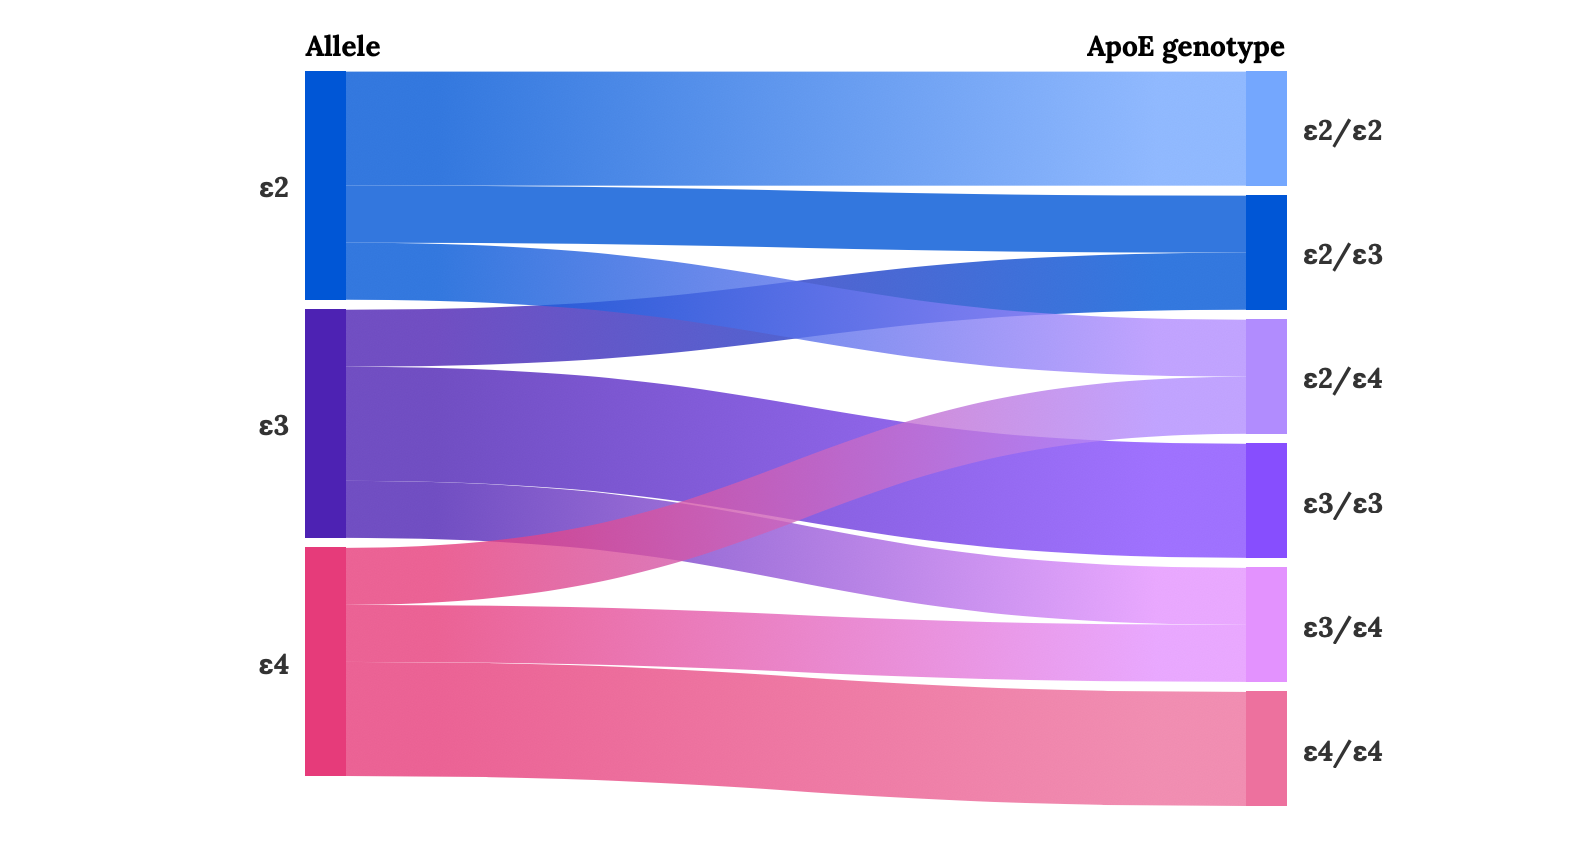
\includegraphics[width=0.7\textwidth]{figures/ApoE@2x.png}
    \caption{Sankey chart showing the allele distribution among the 6 ApoE genotypes.}
  \label{fig1}
\end{figure}

\subsubsection{ApoE and ancestry in Alzheimer's Disease}
The majority of studies exploring the relationship between ApoE alleles and the genetics of LOAD have primarily focused on Northern European populations\cite{Yang2023ApolipoproteinDisease}. However, smaller studies involving diverse ancestral backgrounds show variations in ApoE4 allele \cite{Yang2023ApolipoproteinDisease}. While ApoE4 is present in 14\% of Caucasian Americans, its prevalence increases to 40\% among African Americans, 37\% in Oceania, and 26\% in Australia. Southern Asia and Europe exhibit ApoE4 allelic frequencies of less than 10\%, compared to Northern Europe where it rises to 25\% \cite{Belloy2019AForward, Egert2012ApoEFactors, Eisenberg2010WorldwideHistory, Logue2011AAmericans}.

The epidemiological impact of ApoE alleles also differs among populations. In Korea, Japan, and Japanese-American communities, ApoE4 confers a higher risk of LOAD compared to Caucasians \cite{Farrer1997EffectsMeta-analysis}. Conversely, for Native Americans, Hispanic Americans, African Americans, and those of African descent, ApoE4 is associated with a lower risk of LOAD than in Caucasian-American populations \cite{Farrer1997EffectsMeta-analysis, Blue2019LocalHispanics, Suchy-Dicey2022APOEStudy, Rajabli2018AncestralPopulations, Naslavsky2022GlobalSample}. A recent study in a Chinese population found that ApoE3 is more protective than ApoE2 \cite{Chen2011ApolipoproteinDisease}. Some of these population-specific effects are attributed to the ApoE haplotype \cite{Blue2019LocalHispanics, Rajabli2018AncestralPopulations}. A recent discovery of a novel locus (19q13.31) could contribute to attenuating ApoE4-mediated AD risk in African Americans \cite{Rajabli2022AAncestry}.

\subsubsection{ApoE and sex synergy in Alzheimer's Disease}
Notably, sex (60\% females) and ApoE4 allelic composition (50\% has at least one $\varepsilon_4$ allele) are the strongest genetic risk factors for SAD \cite{, Arnold2020SexMetabolome}. In this regard, it is shown that the ApoE4 genotype has a larger impact on females, as they present greater impairment of mitochondrial energy production, compared to males \cite{Arnold2020SexMetabolome, Yassine2020APOEDisease}.

\subsubsection{Evolution of ApoE over time}
Interestingly, humans are the only species exhibiting polymorphism in the ApoE gene \cite{Yassine2020APOEDisease}. All other animal species have one ApoE variant, which resembles the human ApoE3 allele \cite{Hunsberger2019TheInterventions}. ApoE4 is the oldest human allele, followed by ApoE3 and ApoE2 in age \cite{Yassine2020APOEDisease}. ApoE4 may be adaptive, reducing mortality in highly infectious environments, with food scarcity and shorter lifespans \cite{Trumble2017ApolipoproteinBurden}. However, as human environments became less septic, with food abundance and longer life expectancy, ApoE4 started to burden the arteries and brain, increasing the risk of diseases related to ageing \cite{Yassine2020APOEDisease}. The emergence of ApoE3 from ApoE4 putatively reflects the shift in human diet from a plant-based one to a meat-rich one, where genes adaptive to high meat consumption were and still are vital to regulate increased cholesterol levels \cite{Finch1999TheIsoforms}. 

\subsubsection{Tissue expression}
The principal producers of ApoE are hepatocytes in the liver \cite{Mahley2016CentralMetabolism}. In the CNS, ApoE is primarily expressed in glia, astrocytes, cells of which modulate metabolic homeostasis and neuronal communication, followed by microglia, the brain immune cells \cite{Lanfranco2021ExpressionInflammation}. Each genotype is linked to different expression levels \cite{Husain2021APOETherapeutics}. ApoE2 carriers seem to have higher \acrfull{csf} levels of ApoE, compared to ApoE4 carriers \cite{Castellano2011HumanClearance, Cruchaga2012CerebrospinalDisease}. 

\newpage
\subsection{Apo-lipoprotein E}\label{ApoEprot}
\subsubsection{Structure and function}
\acrshort{apoe} is a brain-specific lipid-binding glycoprotein of 299 amino-acids (34 kDa) that comprises several types of lipoproteins, i.e., chilomicra, \acrlong{idl} and \acrlong{vldl} \cite{Husain2021APOETherapeutics}. Its main function in the brain is the transport of lipids (mainly cholesterol) through membrane receptors \cite{Yang2023ApolipoproteinDisease}. Moreover, its isoforms have an effect on diverse cellular functions, e.g. synaptic integrity, glucose metabolism, A$\beta$ clearance, \acrlong{bbb} integrity and mitochondrial regulation \cite{Husain2021APOETherapeutics}. How these relate to AD pathology will be elaborated in Section \ref{ApoEAD}.



\begin{figure}[htb]
  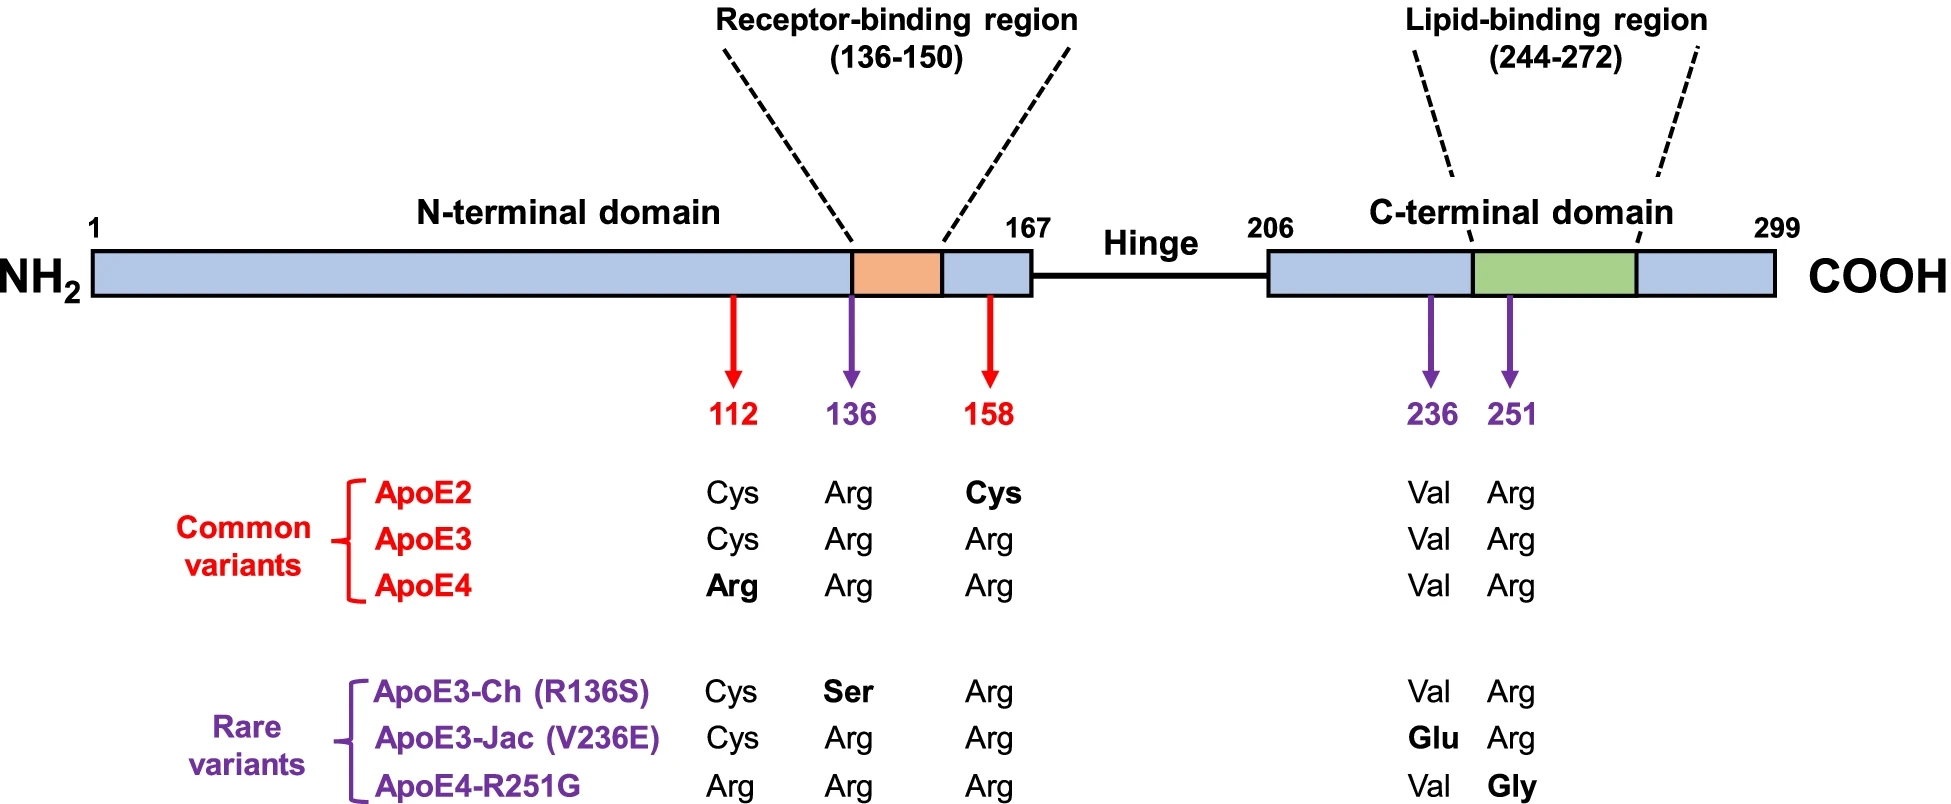
\includegraphics[width=0.8\textwidth]{figures/ApoEprot.png}
    \caption{Linear representation of the ApoE protein. Three structural domains are highlighted: N-terminal, hinge and C-terminal domains. The different aminoacids at positions 112 and 158 are shown per common alleles and aminoacids at positions 136, 236 and 251 coded by rarer alleles. Source: \citetitle{Bu2022APOEVariants}, \Citeauthor{Bu2022APOEVariants} (\citeyear{Bu2022APOEVariants}) \cite{Bu2022APOEVariants}}
  \label{fig2}
\end{figure}

\subsubsection{ApoE isoforms}
The nuances in the amino acid composition of ApoE, specifically the presence of cysteine or arginine at positions 112 and 158, significantly impact its binding with lipids and receptors \cite{Yassine2020APOEDisease}. The most prevalent isoform, ApoE3, features cysteine at position 112 and arginine at position 158  \cite{Yassine2020APOEDisease}, as shown in Fig. \ref{fig2}. ApoE2 has two cysteines, while ApoE4 has two arginines at these positions \cite{Yassine2020APOEDisease}. The C-terminal domain of ApoE (positions 273–299) is crucial for its lipidation specificity and efficiency \cite{Hu2015OpposingMice}.

\subsubsection{Lipidation nuances of ApoE isoforms}
For ApoE to exert its effects, it needs to be lipidated \cite{Husain2021APOETherapeutics}. ApoE undergoes lipidation via \acrfull{abca1}, a lipid efflux protein \cite{Flowers2020APOEBrain, Courtney2016LXRDisease}. The lipidation degree varies among ApoE isoforms, with ApoE4 exhibiting the least efficient lipidation \cite{Hu2015OpposingMice, Heinsinger2016ApolipoproteinFluid}. This discrepancy in lipidation has been linked to alterations in lipoprotein size and type, in that ApoE4 "prefers" large triglyceride-rich VLDL, while ApoE2 and ApoE3 have a higher affinity for phospholipid-rich \acrshort{hdl} particles \cite{Nguyen2010MolecularE4}. The lower affinity of ApoE4 for HDL particles leads to increased levels of unlipidated ApoE, resulting in its aggregation \cite{Hatters2006ApolipoproteinFunction}. Moreover, ApoE4 fibrils are more neurotoxic than those of ApoE2 and ApoE3 \cite{Hatters2006Amino-terminalFibrils}.

Poor lipidation leads to poor ApoE recycling \cite{Yassine2020APOEDisease}. The latter favors the entrapment of ABCA1 in endosomes, away from the cell membrane, thereby pooling cholesterol in the cell membrane rather than attaching it to HDL particles \cite{Rawat2019ApoE4Astrocytes}. This increased cholesterol content in the cell membrane amplifies \acrfull{tlr4} signaling in macrophages, activating \acrshort{nfkb} and inducing an inflammatory gene response \cite{Yassine2020APOEDisease}.  ApoE4 accumulation also sequestrates insulin receptor (IR) in endosomes, impacting cellular energy preferences \cite{Zhao2017ApolipoproteinEndosomes}. This leads to a decrease in glucose utilization for \acrshort{atp} production and an increase in fatty acid oxidation \cite{Svennerholm1997ChangesSwedes}. 

\begin{figure}[t]
  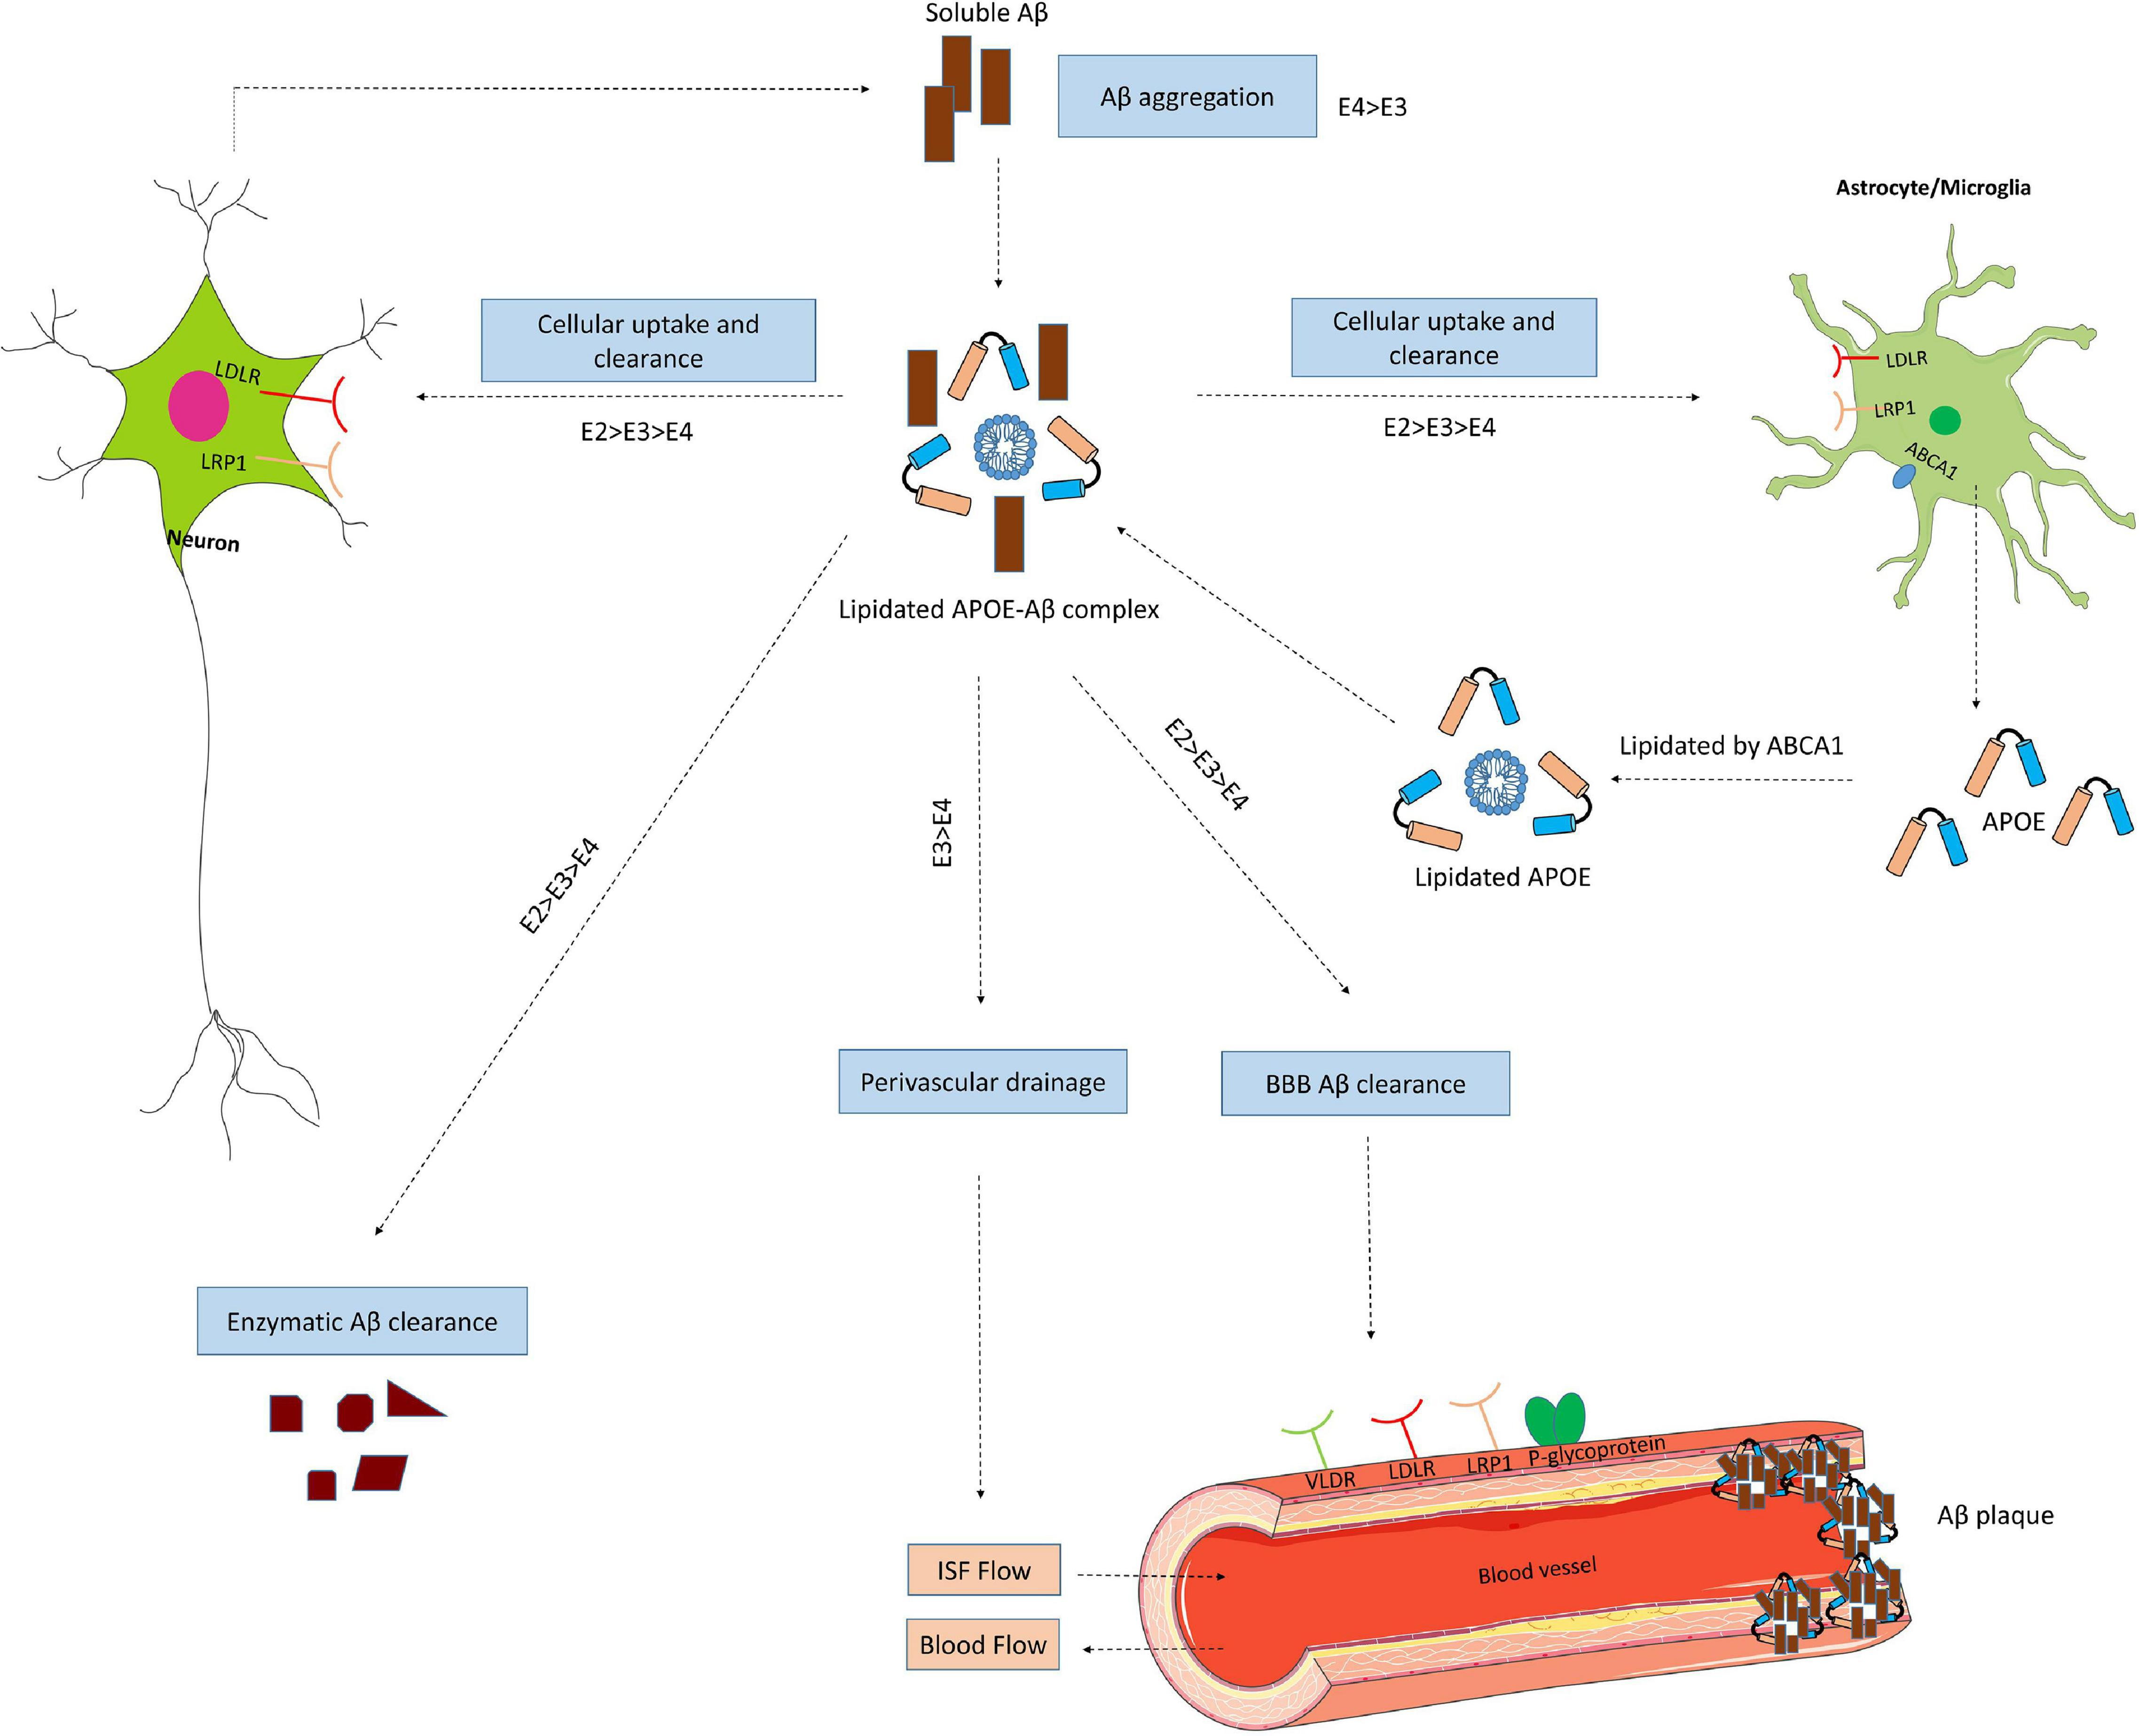
\includegraphics[width=0.8\textwidth]{figures/ApoEeffectsB.jpg}
    \caption{Effects of ApoE isoforms on the metabolism and removal of A$\beta$. A$\beta$ is primarily cleaved from \acrfull{app}. In the brain, ApoE, mainly expressed in astrocytes and microglia, undergoes lipidation by \acrfull{abca1} to create lipoprotein particles. ApoE increases the accumulation and buildup of A$\beta$, or promotes cellular uptake of A$\beta$ by astrocytes or microglia via endocytosis of the lipidated ApoE-A$\beta$ in an isoform-specific manner. This process involves several receptors, such as \acrfull{ldlr} and \acrfull{lrp}. ApoE also facilitates isoform-specific breakdown of A$\beta$ outside the cells. At the \acrlong{bbb}, soluble A$\beta$ is predominantly transported from the \acrfull{isf} into the bloodstream via LRP1 and P-glycoproteins. Additionally, ApoE plays a role in the peri-vascular drainage of A$\beta$. Insufficient clearance of A$\beta$ can lead to its accumulation in the brain tissue, contributing to the formation of A$\beta$ oligomers and amyloid plaques. Source: \citetitle{Husain2021APOETherapeutics}, \Citeauthor{Husain2021APOETherapeutics} (\citeyear{Husain2021APOETherapeutics}) \cite{Husain2021APOETherapeutics}}
  \label{ApoeEffectsA}
\end{figure}

\begin{figure}[b]
  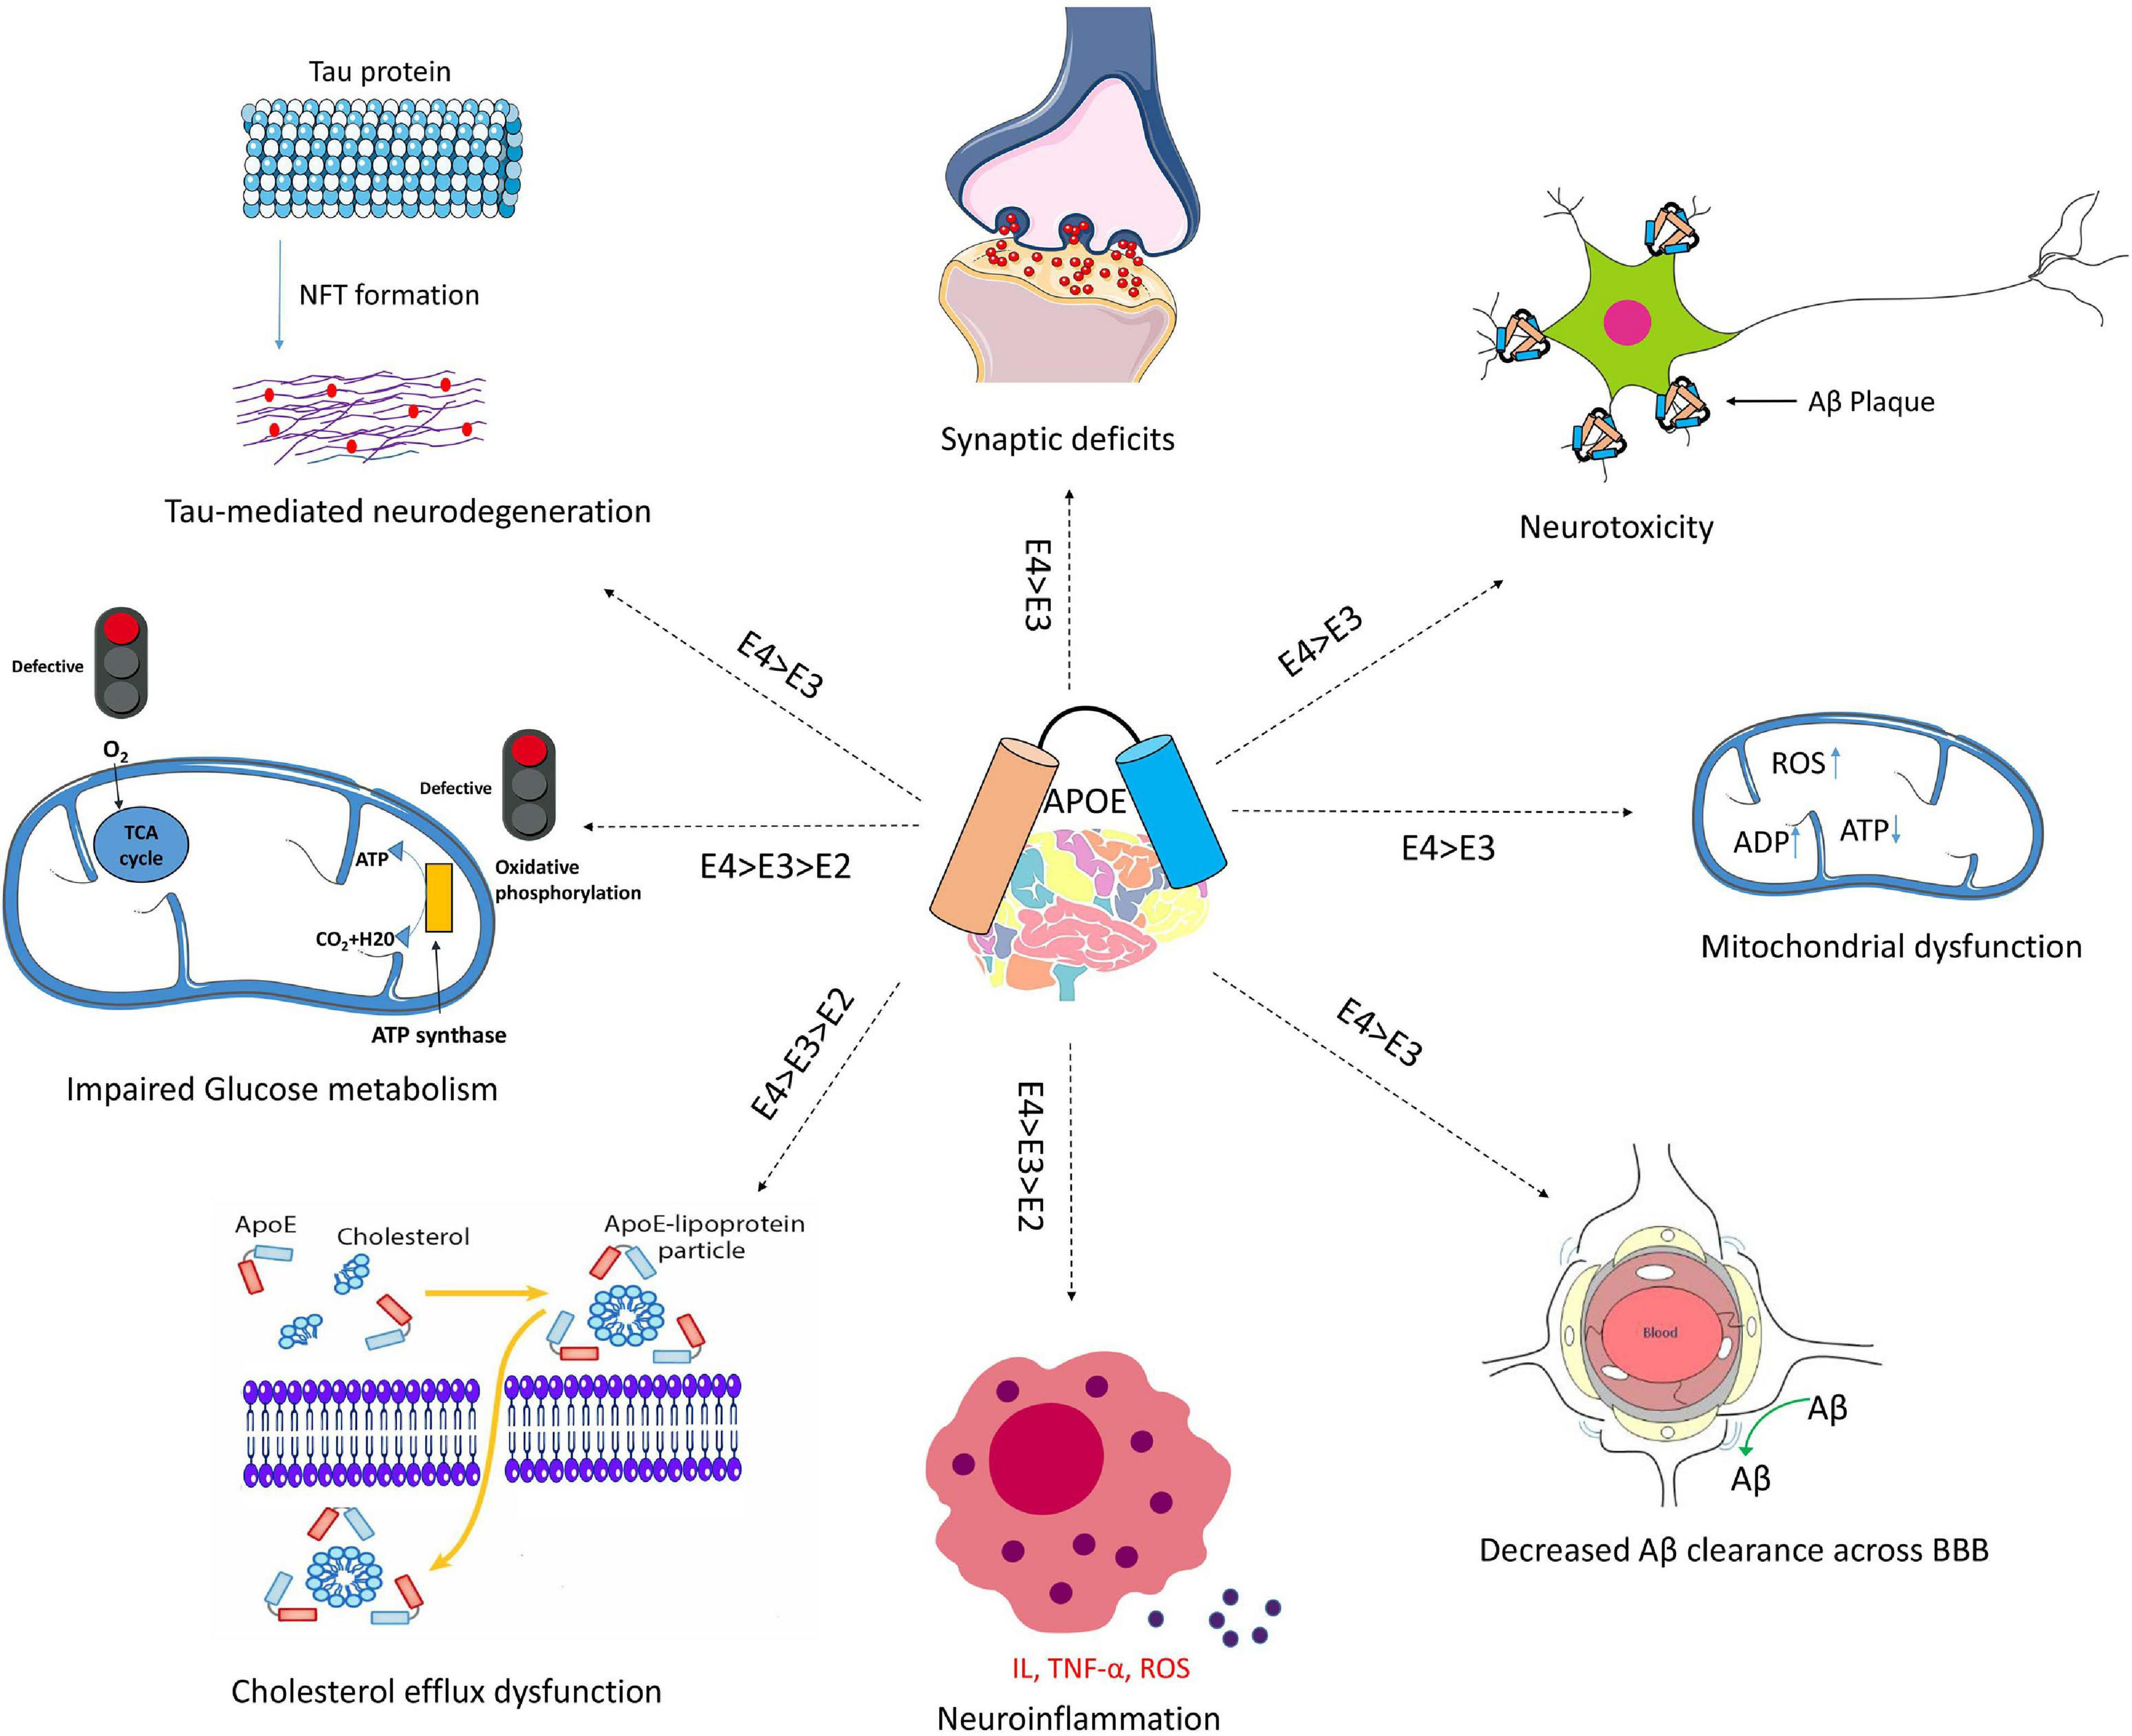
\includegraphics[width=0.8\textwidth]{figures/ApoEeffectsA.jpg}
    \caption{Schematic overview of A$\beta$-independent effects of ApoE in AD pathology. ApoE4 increases the phoshorylation of tau proteins, leading to the creation of tangles, inducing neurodegeneration, synaptic deficits and neurotoxicity. Moreover, ApoE4 is associated with decreased cholesterol efflux and neuroinflammation mediated by \acrfull{il}, \acrfull{tnf}, \acrfull{ros}. In the mitochondria, ApoE4 impairs glucose metabolism and ATP production.  Source: \citetitle{Husain2021APOETherapeutics}, \Citeauthor{Husain2021APOETherapeutics} (\citeyear{Husain2021APOETherapeutics}) \cite{Husain2021APOETherapeutics}}
  \label{ApoeEffectsB}
\end{figure}

\subsubsection{Interplay between ApoE lipidation and Alzheimer's Disease}\label{ApoEAD}
As mentioned earlier, ApoE isoforms have differential pleotropic effects on various cellular functions. ApoE4 induces pro-inflammatory response, leading to the dysfunction of the \acrlong{bbb}, which in turn impairs cognitive functions \cite{Marottoli2017PeripheralDysfunction, Teng2017ApoEInjury, Kloske2020TheDisease}. Moreover, ApoE modulates the primary neuropathological hallmarks of AD: neuroinflammation, A$\beta$ plaques and tau tangles \cite{Husain2021APOETherapeutics}. Evidence from human and transgenic mice studies reveals increased brain A$\beta$ and amyloid plaque loads in ApoE4 carriers, compared to ApoE3; with the lowest levels in ApoE2 carriers \cite{Huang2017ApoE2Secretion, Tachibana2016RescuingLRP1, Safieh2019ApoE4:Disease}. Higher plaque loads are associated with ApoE4 due to its higher affinity for A$\beta$ and poor clearance capacity \cite{Kloske2020TheDisease}. Additionally, high levels of ApoE4 in neurons remarkably increase tau protein phosphorylation, while high concentrations of ApoE3 don't seem to have an effect \cite{Cao2017ApoE4-associatedInjury, Shi2017ApoE4Tauopathy, Vasilevskaya2020InteractionAthletes, Wang2018GainCorrector}. Notably,  ApoE directly inhibits phosphorylation of tau by \acrshort{gsk} \cite{Hoe2006ApolipoproteinNeurons}. An overview of the A$\beta$-independent effects of ApoE is shown in Fig. \ref{ApoeEffectsA}.

\subsection{ApoE4-mediated metabolic changes in Alzheimer's Disease}
Metabolism entails the repertoire of chemical reactions that keep living organisms alive. Metabolites  --especially lipid \cite{Barupal2019SetsPathophysiology,Fernandez-Calle2022APOEDiseases, Proitsi2017AssociationAnalysis}-- , perceived as functional intermediates of AD development, are rigorously studied for bio-markers or targets for treatment \cite{Oeckl2019GlialImpairment}.
 
\subsubsection{Measured in \textit{post-mortem} brain tissue}A metabolomic profiling of brain tissue, obtained \textit{post-mortem} from AD patients and healthy controls showed  pronounced impairments in sterol and sphingolipid levels in ApoE4 carriers with AD  \cite{Bandaru2009ApoE4Brain}. However, another \textit{post-mortem} metabolomic analysis didn't reveal nuances significantly correlated with ApoE4 \cite{Novotny2023MetabolomicBrains}, although they showed trends in increased cholesterol esters, unsaturated lipids, and sphingomyelin species.

\subsubsection{Measured in blood}
Transcriptomic and lipidomic analyses in humanized ApoE mice associated ApoE4 with decreased free fatty acid levels, many increased  tricarboxylic acid (TCA) cycle metabolites, as well as changes in plasma levels of phosphatidylcholines and unsaturated fatty acids \cite{Area-Gomez2020APOE4Mice, Zhao2020AlzheimersPathways}. A recent study on 58 individuals found six downregulated plasma metabolites (including lysophospholipids and cardiolipin) in ApoE4 carriers \cite{pena-bautista2020MetabolomicsEffect}. Further, the plasma metabolome of the latter reveals a preference for aerobic glycolysis \cite{Farmer2021APO4Glycolysis}. Significant correlations of ApoE genotype and sex with metabolites were observed, i.e. several phosphatidylcholines were found in a large study of more than 1500 individuals \cite{Arnold2020SexMetabolome}.

Perturbed serum metabolites associated with AD are aminoacids, amines \cite{deLeeuw2017Blood-basedDisease, Green2023InvestigatingDisease}, cholesteryl esters \cite{Proitsi2017AssociationAnalysis}, sphingolipids \cite{Varma2018BrainStudy,Sun2022AssociationDisease,Green2023InvestigatingDisease,Oeckl2019GlialImpairment,Barupal2019SetsPathophysiology}, fatty acids \cite{Fernandez-Calle2022APOEDiseases,deLeeuw2017Blood-basedDisease}, glycerophospholipids \cite{Varma2018BrainStudy, Jia2022ATypes,Huo2020BrainAnalysis, Weng2019TheImpairment}, phosphatidylcholines \cite{Simpson2016BloodAging} and lipid peroxidation compounds \cite{Fernandez-Calle2022APOEDiseases}. These molecules are usually identified via high-throughput metabolomic pipelines (coupled with Mass Spectrometry (MS) detectors) that trace all compounds in a sample and result in high-dimensional data \cite{Oka2023MultiomicsCohort}. The latter often require advanced statistical methods e.g. projection to latent structures \cite{Weng2019TheImpairment, Peeters2019StableData} or graphical models \cite{Peeters2022Rags2ridges:Matrices} in order to extract putatively meaningful information. 
With such techniques, de Leeuw et al. discovered distinct serum metabolic signatures among AD patients-controls and those carrying at least one ApoE $\varepsilon_4$ allele \cite{deLeeuw2017Blood-basedDisease}, as they appear in Fig. \ref{fig2}. The different metabolic profiles, however, among ApoE4 non-carriers remain obscure. The present data science approach shows ApoE4-mediated differentially expressed metabolites, potentially unveiling distinct pathways of metabolic deregulation in AD.

\begin{figure}[htb]
\vspace*{-0.2cm}
  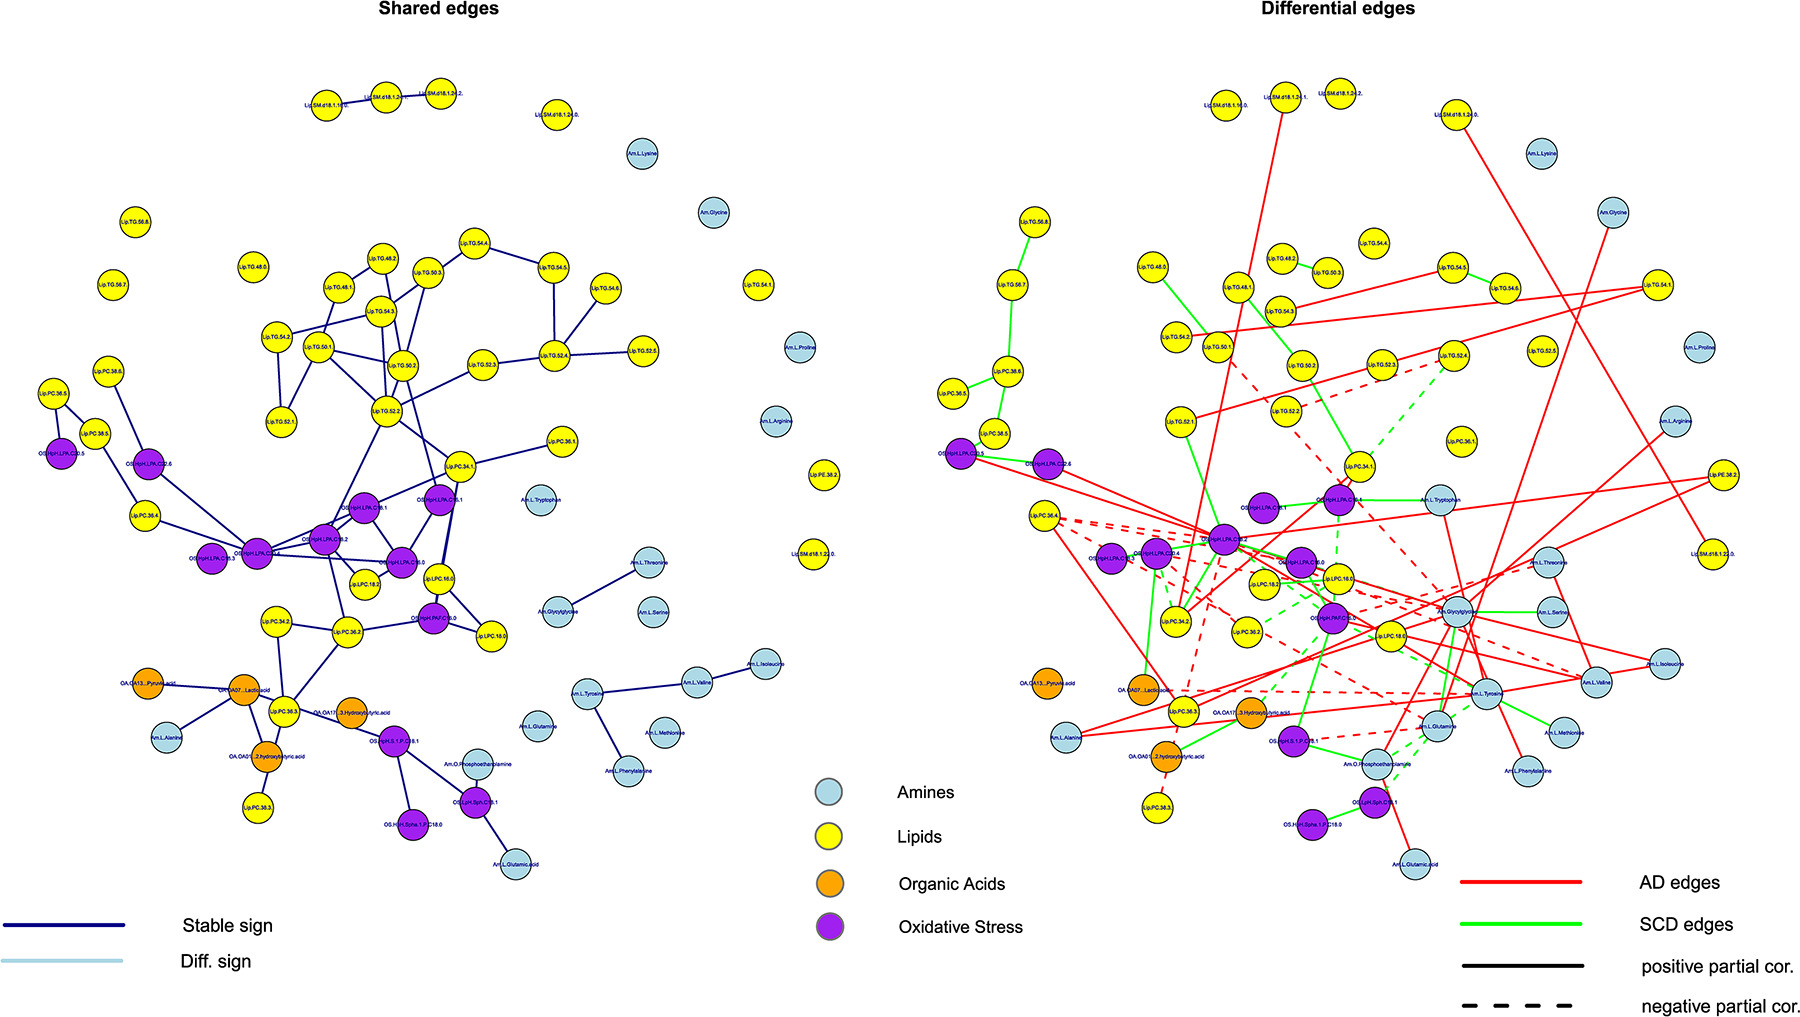
\includegraphics[width=0.9\textwidth]{figures/network.jpeg}
    \caption{Mutual (left-hand panel) and distinct (right-hand panel) metabolic network topologies between ApoE4 carriers and non-carriers in AD, as published by de Leeuw et al.. Red edges represent links that are present exclusively in ApoE4 carriers with AD. Green edges represent connections found in the SCD group. Solid edges represent positive partial correlations, while dashed edges represent negative partial correlations. Abbreviations: SCD, subjective cognitive decline. Source: \citetitle{deLeeuw2017Blood-basedDisease}, \Citeauthor{deLeeuw2017Blood-basedDisease} (\citeyear{deLeeuw2017Blood-basedDisease}) \cite{deLeeuw2017Blood-basedDisease}}
  \label{fig3}
\end{figure}

\newpage
\subsection{Research Questions}
ApoE4 carriers --particularly females-- experience metabolic disturbances and are at increased risk of SAD. The mechanistic links, however, between ApoE4 dose, metabolism and AD development are not entirely known \cite{Fernandez-Calle2022APOEDiseases}. Tracking ApoE4 dose effects on serum metabolites can reveal metabolic perturbations preceding or co-existing with AD. Hence, in an effort to elucidate ApoE4-mediated changes in serum metabolites in AD and SCD, one could state the following research questions (RQ):

Are there mechanistic links between ApoE4 dose and serum metabolome in AD?
\begin{enumerate}
    \item Are there ApoE4 dose effects on serum metabolite levels in AD?
    \item How discriminatory are serum metabolites of ApoE4 status and/or AD?
    \item How do the covariance network topologies of metabolites differ between ApoE4 carriers and non-carriers?
\end{enumerate}

\subsection{Approach and Overview}
An introduction to the data used in this study is found in Section \ref{subjects}. A general overview of the software is found in Section \ref{datamanagement} and \ref{packages}, while the R \texttt{sessionInfo} is found in Appendix \ref{appendixB}. To facilitate statistical analysis, two new features were created for the first two research questions: ApoE4dose (0, 1, 2) and ApoE4AD (4 possible phenotype: AD without ApoE4, AD with at least 1 ApoE4, SCD without ApoE4, SCD with at least 1 ApoE4), respectively, as described in Section \ref{featureeng}.

The statistical methods applied to answer the research questions were adapted from \Citeauthor{deLeeuw2017Blood-basedDisease}'s \citetitle{deLeeuw2017Blood-basedDisease} and are described in Section \ref{stats}. To screen for ApoE4 dose effects on serum metabolites in AD, two approaches were taken: a global test (correcting only for sex) and nested linear model comparison using ANCOVA F-tests (correcting for several factors: Table \ref{tab:clin}, except CSF markers). 

To test the (added) classification potential of serum metabolites against ApoE4AD, several multi-class classification models were fitted. First, a benchmark multinomial logistic regression model was fitted using only clinical background data as predictors. Second, the full metabolomic panel was addded on top of the clinical data in the same model. Third, the metabolites were projected to a latent orthogonal space, where 6 meta-metabolites (accounting for around 30\% of the variance) replaced the original metabolites. Finally, the meta-metabolites were fitted on top of the clinical data in a multinomial logistic regression model, a decision tree and an \acrfull{xgb} model. The discrimatory performance of the aforementioned models was then holistically evaluated and compared.

To visualise and compare the covariance network topologies of metabolites among ApoE4 carriers and non-carriers, the high precision matrices were first sparsified using Ridge and then prunned controlling the False Discrovery Rate. Network topologies were plotted and their statistics were calculated and compared between the ApoE4 carriers and non-carriers using Wilcoxon Signed Rank test.

The results of the analysis are presented in Section \ref{results} and discussed in Section \ref{discuss}.

The study is concluded in Section \ref{concl}


\newpage
\section{Methods}\label{methods}

\subsection{Subjects}\label{subjects}
The data were collected from 126 AD patients and 121 SCD ($n$ = 247) individuals in the context of the Amsterdam Dementia Cohort \cite{VanDerFlier2018AmsterdamCare, deLeeuw2017Blood-basedDisease}. In this study two data sets were used: a targeted metabolomics panel and clinical background data, i.e. age at diagnosis, sex, smoking status, alcohol consumption, hypertension (and medication), hyperlipidemia (and medication), anticoagulant medication, anti-depressants, mean arterial pressure (MAP) and body mass index (BMI) (see Table \ref{tab:clin}). The metabolomics set contains $p =$ 230 metabolites (amines, organic acids, lipids and oxidative stress compounds). The methodology for the metabolomic analysis and ApoE genotyping can be found at de Leeuw et al.'s  Blood-based metabolic signatures in Alzheimer's Disease \cite{deLeeuw2017Blood-basedDisease}: SMT1 . The data was cleaned as described in the same article. The resulting data sets for AD and SCD are high-dimensional, in the sense that they contain more variables than observations ($p > n$). Another particularity of the data is the covariance and collinearity of the variables. Therefore, appropriate measures need to be taken to prevent model over-fitting --the algorithm being unable to distinguish signal from noise and fitting the latter--  and to correct for spurious correlations.

\begin{table}[htb]
\caption{Clinical background characteristics used as control variables of ApoE4 (dose) effects. The molecules measured in CSF were used only in the Multi-class classification. }
\label{tab:clin}
\begin{tabular}{clllll} \toprule
                                & \textbf{Clinical feature}   & \textbf{Type} \\ \midrule
\multirow{2}{*}{Anthropometric} & Age                         & Discrete      \\
                                & Sex                         & Binary        \\
\multirow{2}{*}{Intoxications}  & Smoking (past, current, no) & Nominal       \\
                                & Alcohol                     & Binary        \\
\multirow{3}{*}{Commorbidities} & Hypertension                & Binary        \\
                                & Diabetes mellitus           & Binary        \\
                                & Hypercholesterolemia        & Binary        \\
\multirow{3}{*}{Medication}     & Cholesterol lowering        & Numeric       \\
                                & Antidepressants             & Binary        \\
                                & Antiplatelet                & Binary        \\ 
\multirow{3}{*}{CSF}            & A$\beta_{42}$               & Numeric       \\
                                & tau                         & Numeric       \\
                                & p-tau                       & Numeric       \\\bottomrule
\end{tabular}
\end{table}

\subsection{Data management}\label{datamanagement}
The FAIR principles for data management and stewardship in science were published by  ~\citeauthor{Wilkinson2016TheStewardship} in 2016 \cite{Wilkinson2016TheStewardship}. FAIR stands for Findable, Accessible, Interactive, and Reusable data; the intention is to create and use data that are well-documented and reproducible. These principles were considered at every step of the study and implemented when applicable. The statistical analysis was performed in R (version 4.3.2), and the current report was written in \LaTeX (Tex Live version 2023). All files are stored in a private Github repository --with git as \acrfull{vcs}.

\subsection{Feature Engineering}\label{featureeng}
The ApoE allele and genotype frequencies in the population are reflected in the AD and SCD data, as shown in Table \ref{tab:ApoEfreq}. That is, the most abundant allele is $\varepsilon$3, followed by $\varepsilon4$ and $\varepsilon2$. The most common genotype was $\varepsilon3\varepsilon3$, followed by $\varepsilon3\varepsilon4$ and $\varepsilon4\varepsilon4$.

\begin{table}[htb]
\caption{ApoE genotype counts (top part) ApoE4 counts: features created to balance the genotype counts (bottom part)}
\label{tab:ApoEfreq}
\begin{tabular}{rrccc}
\toprule
\multicolumn{1}{l}{}             & \multicolumn{1}{l}{}       & AD & SCD & Total \\ \midrule
\multirow{6}{*}{ApoE genotypes} & $\varepsilon2\varepsilon$2 & 2  & 0   & 2     \\
                                 & $\varepsilon2\varepsilon3$ & 15 & 3   & 18    \\
                                 & $\varepsilon2\varepsilon4$ & 5  & 2   & 7     \\
                                 & $\varepsilon3\varepsilon3$ & 69 & 37  & 106   \\
                                 & $\varepsilon3\varepsilon4$ & 26 & 59  & 85    \\
                                 & $\varepsilon4\varepsilon4$ & 3  & 26  & 29    \\ \midrule
\multirow{4}{*}{ApoE4 alleles}           & 1x                         & 31 & 61  & 92   \\
                                 & 2x                         & 3  & 26  & 29    \\
                                 & $\geq$ 1x                & 34 & 87  & 121   \\
                                 & No                         & 86 & 40  & 126  \\ \bottomrule
\end{tabular}
\end{table}


The ApoE genotypes is valuable information and might be interesting to screen for metabolic nuances between them. However, the genotypes are not equally represented in the data and hence, testing for differences among them would not be reliable. The following two sections describe the features created to focus on ApoE4 status (0 or at least 1 allele) and dose (0, 1, or 2 alleles) to balance the data when studying only the AD group and both AD and SCD.

\subsubsection{AD group}
\cite{deLeeuw2017Blood-basedDisease} divided the subjects into two classes: those carrying at least one $\varepsilon4$ allele, and $\varepsilon4$ non-carriers. However, in order to study the $\varepsilon4$ \textit{dose} effects, the genotypes can be binned into groups, based on the number of $\varepsilon4$ alleles they carry: 0, 1 or 2. The number of ApoE4 allele doses are shown in the bottom part of Table \ref{tab:ApoEfreq} (first two and last row).

\subsubsection{SCD and AD}
In order to incorporate ApoE4 status, as well as the diagnosis of AD, a four-level feature (AD without ApoE4, AD with at least 1 ApoE4, SCD without ApoE4, SCD with at least 1 ApoE4, "ApoE4AD") was created, as shown in the last two rows of Table \ref{tab:ApoEfreq}.

\subsection{Statistical Analysis} \label{stats}
\subsubsection{ApoE4 dose effects on serum metabolite levels in AD} \label{rq1}
To test if the number of ApoE4 alleles have an effect on mean metabolite levels in AD, two methods were applied: a global test and nested linear model comparison with ANCOVA.

\leavevmode\newline\textbf{Global Test}\hspace{.25cm} The concept of a global test was first introduced by \citeauthor{Simon2004DesignHealth}, and proposed an approach based on permutations to cater to the high dimensionality of gene expression data. The R package \textsf{globaltest} \cite{Goeman2004AOutcome, Goeman2006TestingAlternative, Goeman2023ThePackage} developed by \citeauthor{Goeman2004AOutcome} features a multinomial logistic regression model, fitting genes to predict clinical or biological group membership (number of ApoE4 alleles in this case). This method is also appropriate for other types of -omics data, such as metabolomics in this study \cite{Goeman2023ThePackage}. The null hypothesis is that metabolite levels are independent of the ApoE4 dose X, i.e. $H_0 : P(Y|X) = P(Y)$, where $X \in \mathbb{R}^{n x p}$. The test statistic under $H_0$ follows, asymptotically, a normal distribution. The \texttt{gt} function of the package was used to screen for nuances in metabolite levels on the number of ApoE4 alleles, correcting for sex. To asses ApoE4 dose effects correcting for clinical data nested linear model comparison was performed, as described in the next section.

\leavevmode\newline \textbf{Nested linear models}\hspace{.25cm}
To test for ApoE4 dose effects on each metabolite, $p=230$ model comparisons were needed, hence a function was created to iterate over the metabolites, fit the nested models, compare them using ANCOVA F-tests, store and adjust the p-values, filter those below .05, then consolidate the coefficients of the meaningful full models and the p-values of their t-tests in a table and display it. To decrease run time, as well as harness the power of multiple cores, \textsf{furrr}'s \texttt{future\_map} function was used for parallel iterations.

The dependent variable in each model was a metabolite; the nested model \eqref{rm}, has only clinical variables (Table \ref{tab:clin} except CSF markers) while the full model \eqref{fm}, features the clinical variables, plus the number of ApoE4 alleles (0, 1 or 2 -nominal) as explanatory variables. Let $y_j$ represent the $j$-th metabolite, $x_k$ the $k$-th clinical variable, and $D_{\varepsilon4}$ the ApoE4 dose; the nested models then are:
\begin{align}
    & y_j = \beta_0 + \sum_{k=1}^m\beta_kx_k +\epsilon \label{rm} \\
    & y_j = \beta_0 + \sum_{k=1}^m\beta_kx_k + \beta_{m+1}D_{\varepsilon4} + \epsilon \label{fm}
\end{align}
For every metabolite $j$ = 1,...,$p$ the hypothesis test is 
H$_0$: $\beta_{m+1} = 0 $ vs H$_\alpha$: $\beta_{m+1} \neq 0$.
Under H$_0$ the test statistic, $F$ follows an $F_{1, n-(m+2)}$ distribution. This implies $p$ hypothesis tests, which qualifies as multiple testing. A method to treat the latter is controlling False Discovery Rate \cite{Benjamini1995ControllingTesting}, that is controlling the expected ratio of incorrectly rejected H$_0$ hypotheses, globally e.g. at an $\alpha$ of 0.05. First, the p-values are sorted in ascending order, and for every $j$ p-value each $\alpha$ is multiplied by $j$ divided by the total number of p-values \cite{Benjamini1995ControllingTesting} $m = 230$ in this study. In other words, after adjustment, a null hypothesis $j$ may be rejected only if its associated F-test's p-value is less than a fraction ($j/m$) of $\alpha$.

\begin{algorithm}
\caption{Benjamini–Hochberg's procedure to control FDR}\label{alg:fdr}
Specify $\alpha$, the level at which to control the FDR.\\
Compute p-values, $p_1, ... , p_m$, for the $m$ null hypotheses $H_{01},...,H_{0m}$. \\
Order the $m$ p-values so that $p(1) \leq p(2) \leq ... \leq p(m)$.\\
Define
\[L = \max\{j : p(j) \leq \frac{j}{m}\alpha\}\] \\
Reject all null hypotheses $H_{0j}$ for which $p_j \leq p(L)$.
\end{algorithm}

\subsubsection{Classification of ApoE4 status and/or AD}\label{rq2}
In machine learning, a class denotes a group of objects that share common characteristics, such as having AD or ApoE4 \cite*{Drummond2010}. Classification, in this context, denotes training a (supervised) learning algorithm on labeled data (containing their class) \cite*{Drummond2010}. The classifier learns patterns in the data and is then able to predict class membership for unknown data \cite*{Drummond2010}.

\leavevmode\newline \textbf{Bias-Variance trade-off}\hspace{.25cm}The degree to which a user can understand and interpret the prediction or decisions made by a statistical model is defined as \textit{interpretability} \cite{Elshawi2019OnHypertension}. It is of interest in this study to find the optimal balance between the performance of a model with its interpretability. The \textit{bias-variance trade-off} was formally introduced by \citeauthor{Geman1992NeuralDilemma} and refers to the trade-off between the accuracy (opposite of bias) and precision (opposite of variance) of a prediction. It also refers to the trade-off between model flexibility (or complexity) and interpretability \cite{Geman1992NeuralDilemma}. One may consider this trade-off during model and evaluation method selection, as some impose more bias or variance than others.

\leavevmode\newline \textbf{Multi-class classification models}\hspace{.25cm}The R package \textsf{caret} streamlines the training and comparison of classification and regression models, offering broad parametrization options \cite{Kuhn2008BuildingPackage}. The functions \texttt{trainControl} and \texttt{train} were used to fit the models. A sampling method used to deal with the unbalanced classes was \acrshort{smote} (Synthetic Minority Over-Sampling Technique), as implemented by the package \textsf{DMwR2} \cite{DMwR2}.

Considering interpretability, Multinomial Logistic Regression (\acrshort{mnl}) is inherently interpretable. Let $y = k$, with $k \in N, [1,4]$ representing the k-th class of ApoE4AD and $\beta_{kj}$ its set of coefficients,  $\beta_{lj}$ the coefficients of the rest of classes for $j$-th metabolite, then a MNL model calculated the probability

\[\textrm{Pr}(y=k|X=x) =  \dfrac{e^{\sum_{j=1}^{p}\beta_{kj}x_j}}{\sum_{l=1}^{4}\sum_{j=1}^{p}e^{\beta_{lj}x_j}}\]

When $p > n$, the coefficient estimation method has low bias and high variance, in that small changes in the training data can result in very different coefficient estimates \cite{James2023AnEdition}. Regularization trades off a small increase in bias for a great decrease in variance, by shrinking the unimportant coefficients towards zero. \acrshort{lasso} (Least Absolute Shrinkage and Selection Operator) \cite{Tibshiranit1996RegressionLasso}, also called L1-regularization shrinks the MNL coefficients to 0, thus weeding out spurious correlations and reducing the number of predictors \cite{Tibshiranit1996RegressionLasso}. It does so by introducing the term  \[\lambda\sum_{j=1}^{p}|\beta_j|\] where $\lambda \geq 0$ is a tuning parameter that balances the coefficient shrinking effect. The package \textsf{nnet}, as implemented in \textsf{caret}'s \texttt{train} function was used in this case.

A method to treat multi-collinearity and high dimensionality is a 2-stage \acrfull{ml} \acrfull{fa}, such as the one the package \textsf{FMradio} \cite{Peeters2019StableData} performs. In the 1st stage, a L2-regularised ML estimation is used to filter out redundant features from the data matrix. In the second stage, ML FA projects the aforementioned matrix to an orthogonal space where the features are replaced by -fewer- factors that explain their covariance. One can then use the produced factor scores as predictors in MNL.

Decision Trees (DT) are inherently interpretable, non-parametric models, that fit well large and complicated data sets. They have a tree-like structure that splits the data into branches and leaves(nodes) \cite{Song2015DecisionPrediction}. The \texttt{rpart2} \cite{rpart} function of \textsf{rpart} was used.

Boosting models, are ensemble models that fit several weak learners (such as linear/logistic regression or DTs) sequentially, reweighing the data, and take their weighted majority vote \cite{Friedman2000boosting,Friedman2001gbm}. Despite Boosting tends to outperform DTs, it often operates as a \textit{black box} and is poorly interpretable. The state-of-the-art \acrlong{xgb} (\texttt{xgbTree}) of the package \textsf{xgboost} \cite{Chen2016XGBoost:System} was used.

\begin{algorithm}
\caption{Multi-class classification of ApoE4 and AD status pipeline} \label{alg:classification}
    Fit clinical data only in MNL\\
    Fit clinical data + 230 serum metabolites in MNL\\
    Fit clinical data + 6 meta-metabolites in MNL\\
    Fit clinical data + 6 meta-metabolites in a Decision Tree\\
    Fit clinical data + 6 meta-metabolites in an XGBoost\\
    Evaluate performance and compare
\end{algorithm}

First, a benchmark model was created fitting the clinical background data to predict ApoE4AD in a penalised MNL model. Second, the 230-metabolite panel was fitted on top of the clinical background data in a penalised MNL model. Then the full metabolite panel was projected into 6 latent factors (meta-metabolites), explaining around 30\% of their variance. The 6-factor metabolite projection was then fitted on top of the clinical data in a penalised MNL, a DT and an XGBoost model. The aforementioned models were hyper-parameter tuned over a grid of values and the best was selected using repeated (100 times) 10-fold Cross-Validation (CV). 

Model performance was holistically assessed and compared, with the repeated 10-fold CV-obtained ROC curves and their respective Area Under the Curve \acrshort{auc} using the \textsf{pROC} package \cite{pROC} and other metrics such as Accuracy, Precision, Recall and F1-score from \textsf{caret}'s \texttt{confusionMatrix}.

\subsubsection{Metabolite Covariance Network Analysis}\label{rq3}
Network science offers a unifying framework for data and system representation, applicable to any domain \cite{Barabasi2015NetworkScience}. A network, in an abstract sense, consists of nodes connected with links, also referred to as edges. In data science, a network whose nodes represent random features, whose joint probability distribution is defined by the ensemble of their edges is called \textit{graphical model} \cite{Peeters2022Rags2ridges:Matrices}. A metabolomic covariance correlation network represents the ensemble of metabolites based on their covariance, showing nuances among the samples that non-graphical statistical methods on individual metabolites may fail to detect \cite{PerezDeSouza2020Network-basedInterpretation}. It may provide insights into correlated metabolites that don't belong in the same metabolic pathway \cite{PerezDeSouza2020Network-basedInterpretation}.


A \textit{Gaussian graphical model} (\acrshort{ggm}) is an undirected graph that represents the conditional independence properties of the features \cite{KollerProbabilisticTechniques}. The statistic employed by GGMs is the partial correlation which also adjusts for indirect correlation, i.e. two metabolites are correlated with a third one and are shown correlated with each other \cite{Amara2022NetworksInterpretation}. For instance, let $\mathcal{G=(V,E)}$ be a GGM consisting of a set $\mathcal{V}$ of $p$ vertices, corresponding to random features $Y_1,...,Y_p$ with joint probability distribution $P \sim N_p(\mathbf{0, \Sigma})$, and set of edges $\mathcal{E}$, such that for all pairs $\{Y_i , Y_j\}$ with $i\neq j$:

\[ \mathbf{\Sigma}_{ij}^{-1} = (\mathbf{\Omega}_{ij})=0 \Longleftrightarrow Y_i \Perp Y_j\mid\{Y_k : k \neq i,j\} \Longleftrightarrow (i, j) \notin \mathcal{E} \]

In natural language, a zero value in the inverse covariance matrix (usually referred to as precision matrix $\mathbf{\Omega}$) implies that the respective random features are independent, given the rest of features, and they are not connected by an undirected edge $((i, j) \notin \mathcal{E})$ \cite{Peeters2022Rags2ridges:Matrices}.

In this study, the package \textsf{rags2ridges} \cite{Peeters2022Rags2ridges:Matrices} was used to generate the feature covariance matrix, as well as the precision matrix, regularise it and represent it in a GGM --as shown in Fig. \ref{fig2}.

\subsection{R packages} \label{packages}
\hspace{5 pt}
\begin{multicols}{3}
\begin{itemize}
    \item[] \textsf{caret} \cite{Kuhn2008BuildingPackage}
    \item[]\textsf{dplyr} \cite{dplyr}
    \item[]\textsf{DMwR2} \cite{DMwR2}
    \item[]\textsf{globaltest} \cite{Goeman2004AOutcome, Goeman2006TestingAlternative, Goeman2023ThePackage}
    \item[]\textsf{heatmaply} \cite{heatmaply}
    \item[]\textsf{FMradio} \cite{Peeters2019StableData}
    \item[]\textsf{nnet} \cite{nnet}
    \item[]\textsf{pROC} \cite{pROC}
    \item[]\textsf{rags2ridges} \cite{Peeters2022Rags2ridges:Matrices}
    \item[]\textsf{rpart} \cite{rpart}
    \item[]\textsf{xgboost} \cite{Chen2016XGBoost:System}
    \item[]\textsf{furrr} \cite{furrr}
\end{itemize}
\end{multicols}

\clearpage
\section{Results} \label{results}
\subsection{ApoE4 dose effects on serum metabolite levels in AD}
\subsubsection{Global Test}
Testing for ApoE4 dose-effect on serum metabolites of AD patients, correcting for sex (Ho: ApoE4 dose has no effect on mean metabolite levels, Ha: it has an effect), showed a significant global difference in metabolites (p = 0.017). The most significantly affected metabolites are triglycerides and diglycerides (FDR-adjusted p-value $<$0.05) See Table \ref{tab:gt} and Fig. \ref{plot:gt}.

\begin{table}
  \centering
  \caption{Metabolites affected by ApoE4 dose, correcting for sex as per globaltest \cite{Goeman2023ThePackage}}
  \label{tab:gt}
  \begin{tabular}{lrcrr} \toprule
                         & \multicolumn{1}{l}{Inheritance} & Assoc. with & \multicolumn{1}{l}{p-value} & \multicolumn{1}{l}{FDR}  \\ \midrule
  Lip.TG.56.2.           & 0.046                           & 1 ApoE4     & $<$0.001                           & 0.016                    \\
  Lip.TG.58.1.           & 0.117                           & 1 ApoE4     & $<$0.001                           & 0.021                    \\
  Lip.DG.36.3.           & 0.19                            & 1 ApoE4     & $<$0.001                           & 0.021                    \\
  Lip.TG.56.3.           & 0.244                           & 1 ApoE4     & $<$0.001                           & 0.021                    \\
  Lip.TG.52.3.           & 0.424                           & 1 ApoE4     & 0.001                       & 0.031                    \\
  Lip.TG.54.5.           & 0.48                            & 1 ApoE4     & 0.001                       & 0.027                    \\
  Lip.TG.58.2.           & 0.722                           & 1 ApoE4     & 0.001                       & 0.027                    \\
  Lip.TG.54.4.           & 0.761                           & 1 ApoE4     & 0.002                       & 0.033                    \\
  Lip.TG.58.9.           & 1                               & 1 ApoE4     & 0.001                       & 0.027                    \\
  Lip.TG.56.7.           & 1                               & 1 ApoE4     & 0.001                       & 0.027                    \\
  Lip.TG.58.8.           & 1                               & 1 ApoE4     & 0.001                       & 0.032                    \\
  Lip.TG.54.6.           & 1                               & 1 ApoE4     & 0.002                       & 0.035                    \\
  Lip.TG.56.8.           & 1                               & 1 ApoE4     & 0.002                       & 0.037                    \\
  Lip.TG.52.4.           & 1                               & 1 ApoE4     & 0.003                       & 0.055                    \\
  Lip.TG.54.3.           & 1                               & 1 ApoE4     & 0.004                       & 0.055                    \\
  Lip.TG.56.6.           & 1                               & 1 ApoE4     & 0.004                       & 0.059                    \\
  Lip.TG.56.1.           & 1                               & 1 ApoE4     & 0.004                       & 0.059                    \\
  Lip.TG.52.2.           & 1                               & 1 ApoE4     & 0.005                       & 0.063                    \\
  Lip.TG.54.2.           & 1                               & 1 ApoE4     & 0.005                       & 0.063                    \\
  Lip.TG.60.2.           & 1                               & 1 ApoE4     & 0.007                       & 0.077                    \\
  Lip.TG.58.10.          & 1                               & 1 ApoE4     & 0.011                       & 0.124                    \\
  Lip.TG.51.3.           & 1                               & 1 ApoE4     & 0.015                       & 0.154                    \\
  Lip.SM.d18.1.18.1.     & 1                               & 2 ApoE4     & 0.018                       & 0.169                    \\
  OA.2.ketoglutaric.acid & 1                               & 2 ApoE4     & 0.019                       & 0.169                    \\
  Lip.TG.52.0.           & 1                               & 1 ApoE4     & 0.019                       & 0.169                    \\
  Lip.TG.50.3.           & 1                               & 2 ApoE4     & 0.02                        & 0.169                    \\
  OA.Uracil              & 1                               & no ApoE4    & 0.02                        & 0.169                    \\
  Lip.TG.52.5.           & 1                               & 1 ApoE4     & 0.021                       & 0.174                    \\
  Lip.TG.54.0.           & 1                               & 1 ApoE4     & 0.022                       & 0.174                    \\
  Lip.TG.50.2.           & 1                               & 2 ApoE4     & 0.022                       & 0.174                    \\
  Lip.TG.51.2.           & 1                               & 1 ApoE4     & 0.023                       & 0.174                    \\
  Am.L.Glutamine         & 1                               & no ApoE4    & 0.024                       & 0.174                    \\
  Lip.TG.50.1.           & 1                               & 2 ApoE4     & 0.025                       & 0.174                    \\
  Lip.TG.50.4.           & 1                               & 1 ApoE4     & 0.026                       & 0.176                    \\
  Lip.TG.52.1.           & 1                               & 1 ApoE4     & 0.027                       & 0.176                    \\
  Lip.TG.54.1.           & 1                               & 1 ApoE4     & 0.031                       & 0.203                    \\
  Lip.TG.50.0.           & 1                               & 1 ApoE4     & 0.037                       & 0.229                    \\
  OA.Malic.acid          & 1                               & 2 ApoE4     & 0.038                       & 0.234                    \\
  Lip.DG.36.2.           & 1                               & 1 ApoE4     & 0.039                       & 0.235                    \\
  OS.HpH.PAF.C16.0       & 1                               & 2 ApoE4     & 0.049                       & 0.283                 \\ \bottomrule  
  \end{tabular}
  \end{table}


\begin{figure}[htb]
    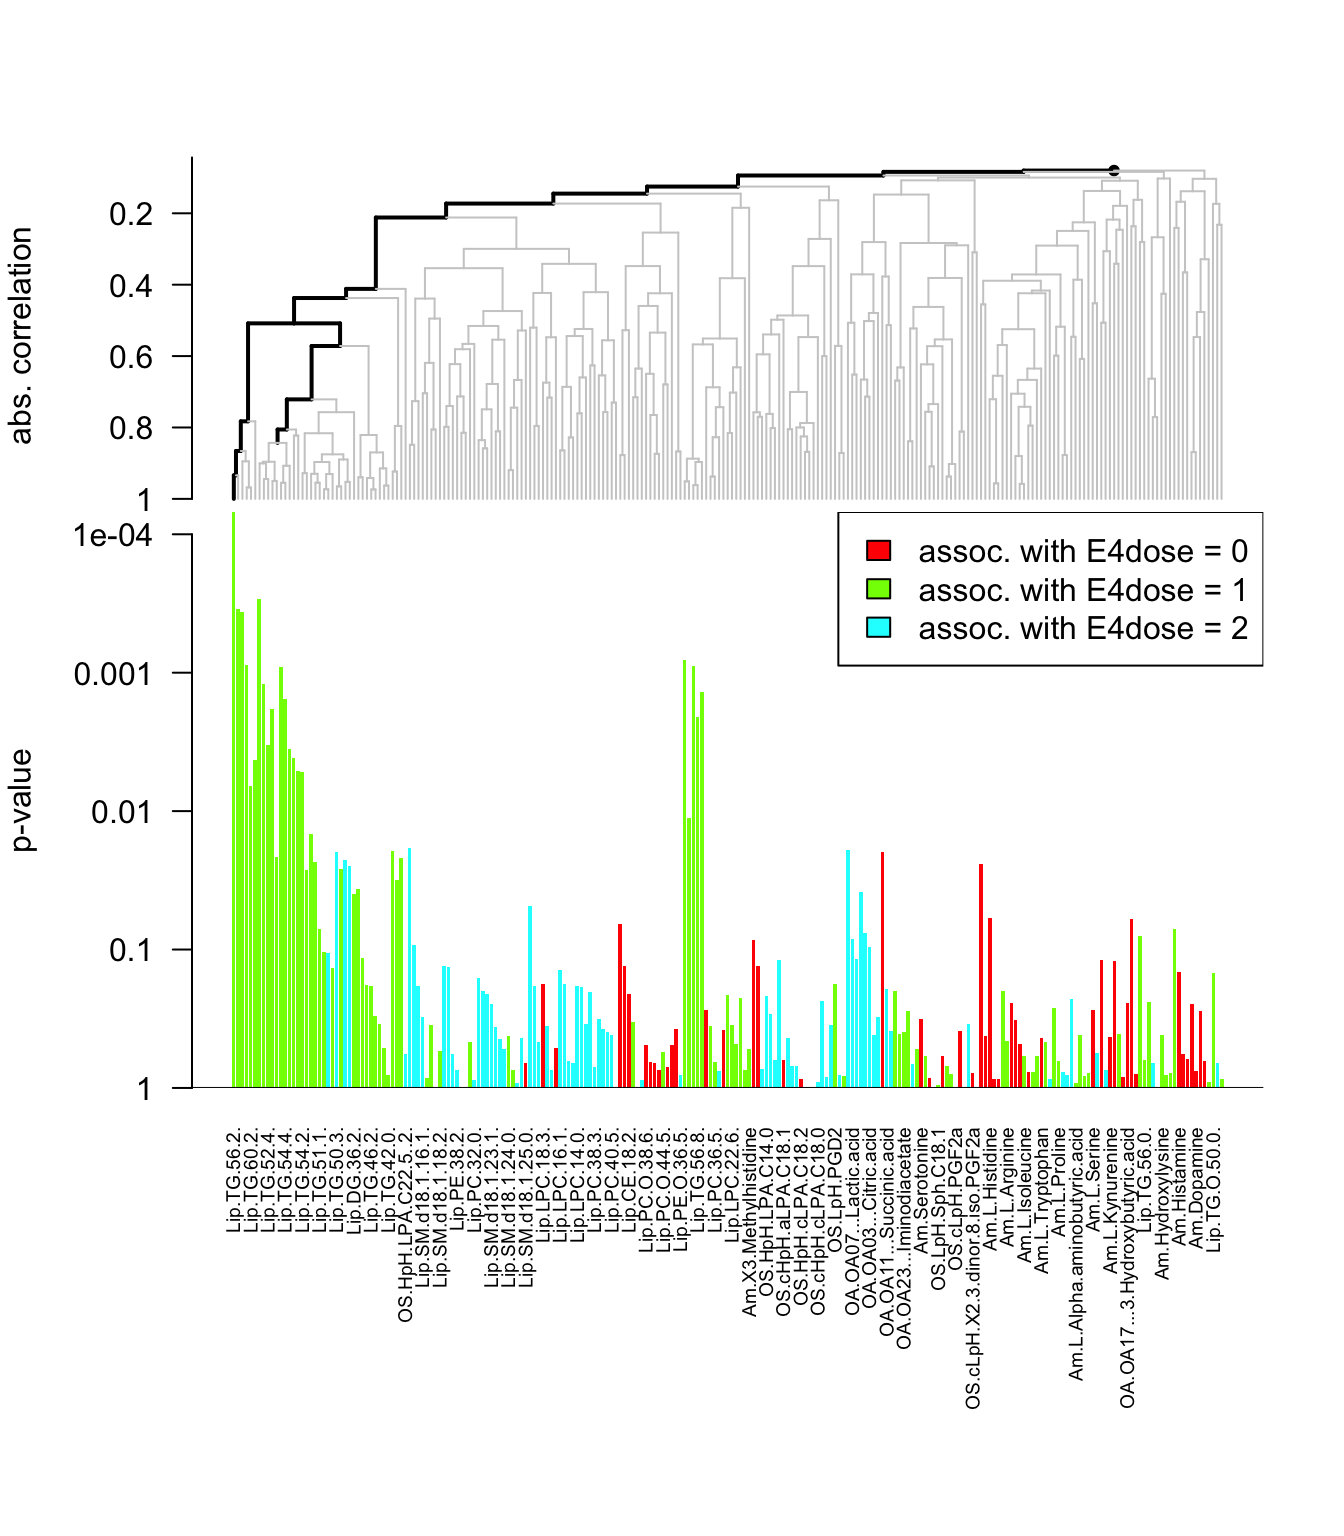
\includegraphics[width=0.9\textwidth]{figures/gt2.png}
      \caption{Covariates plot showing the metabolites affected by the number of ApoE4 alleles}
    \label{plot:gt}
  \end{figure}
\clearpage  
\subsubsection{Nested Linear Models}
Several metabolites from all classes were affected by ApoE4 dose, both in AD and SCD however, after correcting for multiple testing by controlling FDR, none of the effects were significant at $\alpha=0.05$. Among AD patients, ApoE4 dose seems to have positive effect on several triglycerides, diglycerides, putrescine, 2-ketoglutraric acid, lysophosphatidylcholin, HpH.PAF.-C16.0 and -C18.0 (Table \ref{tab:nestedF}). Among individuals with SCD, lipid metabolites were not affected as much as in the AD group, with only two sphingomyelin species showing a difference. Aminoacids L-serine, tryptophan, glycine,trytptophan, L-homoserine, putrescine were affected in this group. L-Tryptophan is negatively associated with ApoE4 dose (at 1x and 2x ApoE4), while L-serine, glycine and L-homoserine are negativelly associated only with ApoE4 homozygotes. (Table \ref{tab:nestedF}). 
\begin{table}[H]
\caption{ApoE4 dose effects on metabolites in AD and SCD: significant F tests ($\alpha=0.05$) from nested linear model comparison. Reduced model: \eqref{rm}, Full model: \eqref{fm}. Am: Aminoacid, Lip: Lipid, DG: Diglyceride, LPC: Lysophosphatidylcholine, SM: Sphingomyelin, TG: Triglyceride, OA: Organic Acid, OS: Oxidative Stress compound}
\label{tab:nestedF}
\centering
  \begin{tabular}{clrrrrrrrr} \toprule
    \multicolumn{1}{l}{} & \multicolumn{1}{c}{\multirow{2}{*}{Metabolite}} & \multicolumn{1}{c}{\multirow{2}{*}{P($>$F)}} & \multicolumn{1}{c}{\multirow{2}{*}{FDR}} & \multicolumn{2}{c}{No $\varepsilon4$} & \multicolumn{2}{c}{1x $\varepsilon4$} & \multicolumn{2}{c}{2x $\varepsilon4$} \\
\multicolumn{1}{l}{} & \multicolumn{1}{c}{} & \multicolumn{1}{c}{} & \multicolumn{1}{c}{} & \multicolumn{1}{l}{Coef.} & \multicolumn{1}{l}{P($>$t)} & \multicolumn{1}{l}{Coef.} & \multicolumn{1}{l}{P($>$t)} & \multicolumn{1}{l}{Coef.} & \multicolumn{1}{l}{P($>$t)} \\ \midrule
  % \multicolumn{1}{l}{} & Metabolite & \multicolumn{1}{l}{P($>$F)} & \multicolumn{1}{l}{FDR} & \multicolumn{1}{l}{No $\varepsilon4$} & \multicolumn{1}{l}{P($>$t)} & \multicolumn{1}{l}{1x$\varepsilon4$} & \multicolumn{1}{l}{P($>$t)} & \multicolumn{1}{l}{2x$\varepsilon4$} & \multicolumn{1}{l}{P($>$t)} \\ 
  \multirow{19}{*}{AD} & Lip.TG.52.3. & 0.001 & 0.156 & {\cellcolor[rgb]{0.98,0.8,0.808}}-1.4 & 0.818 & {\cellcolor[rgb]{0.949,0.973,0.969}}2.6 & 0.004 & {\cellcolor[rgb]{0.929,0.965,0.949}}3.7 & 0.001 \\
   & Lip.TG.52.4. & 0.003 & 0.156 & {\cellcolor[rgb]{0.984,0.988,0.996}}0.6 & 0.888 & {\cellcolor[rgb]{0.969,0.98,0.98}}1.6 & 0.008 & {\cellcolor[rgb]{0.953,0.976,0.973}}2.4 & 0.002 \\
   & Lip.DG.36.3. & 0.002 & 0.156 & {\cellcolor[rgb]{0.984,0.957,0.969}}0.0 & 0.631 & {\cellcolor[rgb]{0.984,0.957,0.965}}0.0 & 0.012 & {\cellcolor[rgb]{0.984,0.957,0.969}}0.0 & 0.001 \\
   & OS.HpH.PAF.C16.0 & 0.002 & 0.156 & {\cellcolor[rgb]{0.388,0.745,0.482}}34.8 & $<$0.001 & {\cellcolor[rgb]{0.949,0.973,0.969}}2.6 & 0.017 & {\cellcolor[rgb]{0.914,0.961,0.937}}4.6 & 0.001 \\
   & Lip.TG.52.2. & 0.006 & 0.255 & {\cellcolor[rgb]{0.973,0.412,0.42}}-5.1 & 0.469 & {\cellcolor[rgb]{0.957,0.976,0.976}}2.1 & 0.03 & {\cellcolor[rgb]{0.929,0.965,0.949}}3.7 & 0.002 \\
   & Lip.TG.54.5. & 0.01 & 0.373 & {\cellcolor[rgb]{0.965,0.98,0.98}}1.9 & 0.496 & {\cellcolor[rgb]{0.98,0.984,0.992}}0.9 & 0.016 & {\cellcolor[rgb]{0.973,0.984,0.988}}1.3 & 0.006 \\
   & Lip.TG.50.2. & 0.012 & 0.398 & {\cellcolor[rgb]{0.973,0.471,0.478}}-4.5 & 0.297 & {\cellcolor[rgb]{0.98,0.984,0.992}}0.9 & 0.141 & {\cellcolor[rgb]{0.957,0.976,0.973}}2.2 & 0.003 \\
   & Lip.TG.50.1. & 0.018 & 0.45 & {\cellcolor[rgb]{0.98,0.706,0.714}}-2.3 & 0.539 & {\cellcolor[rgb]{0.984,0.988,0.996}}0.7 & 0.179 & {\cellcolor[rgb]{0.965,0.98,0.98}}1.8 & 0.005 \\
   & Lip.TG.54.4. & 0.02 & 0.45 & {\cellcolor[rgb]{0.937,0.969,0.953}}3.5 & 0.318 & {\cellcolor[rgb]{0.976,0.984,0.988}}1.2 & 0.015 & {\cellcolor[rgb]{0.973,0.984,0.984}}1.4 & 0.02 \\
   & Lip.TG.54.6. & 0.017 & 0.45 & {\cellcolor[rgb]{0.984,0.906,0.918}}-0.4 & 0.795 & {\cellcolor[rgb]{0.988,0.988,1}}0.5 & 0.027 & {\cellcolor[rgb]{0.984,0.988,0.996}}0.7 & 0.009 \\
   & Am.Putrescine & 0.029 & 0.515 & {\cellcolor[rgb]{0.984,0.953,0.965}}0.0 & $<$0.001 & {\cellcolor[rgb]{0.984,0.953,0.965}}0.0 & 0.035 & {\cellcolor[rgb]{0.984,0.953,0.965}}0.0 & 0.017 \\
   & OA.2.ketoglutaric.acid & 0.026 & 0.515 & {\cellcolor[rgb]{0.984,0.953,0.965}}0.0 & 0.366 & {\cellcolor[rgb]{0.984,0.953,0.965}}0.0 & 0.953 & {\cellcolor[rgb]{0.984,0.953,0.965}}0.0 & 0.014 \\
   & Lip.TG.50.3. & 0.028 & 0.515 & {\cellcolor[rgb]{0.98,0.824,0.835}}-1.2 & 0.668 & {\cellcolor[rgb]{0.984,0.988,0.996}}0.6 & 0.127 & {\cellcolor[rgb]{0.973,0.984,0.988}}1.3 & 0.008 \\
   & Lip.TG.52.5. & 0.042 & 0.538 & {\cellcolor[rgb]{0.988,0.988,1}}0.5 & 0.789 & {\cellcolor[rgb]{0.988,0.988,1}}0.4 & 0.134 & {\cellcolor[rgb]{0.984,0.988,0.996}}0.7 & 0.014 \\
   & Lip.TG.56.7. & 0.042 & 0.538 & {\cellcolor[rgb]{0.976,0.698,0.706}}-2.4 & 0.095 & {\cellcolor[rgb]{0.988,0.988,1}}0.5 & 0.015 & {\cellcolor[rgb]{0.988,0.988,1}}0.4 & 0.105 \\
   & Lip.TG.56.8. & 0.044 & 0.538 & {\cellcolor[rgb]{0.98,0.804,0.816}}-1.4 & 0.055 & {\cellcolor[rgb]{0.984,0.98,0.992}}0.2 & 0.014 & {\cellcolor[rgb]{0.984,0.973,0.984}}0.2 & 0.151 \\
   & Lip.TG.58.9. & 0.042 & 0.538 & {\cellcolor[rgb]{0.984,0.906,0.918}}-0.4 & 0.068 & {\cellcolor[rgb]{0.984,0.961,0.973}}0.1 & 0.013 & {\cellcolor[rgb]{0.984,0.957,0.969}}0.0 & 0.41 \\
   & Lip.LPC.16.0. & 0.033 & 0.538 & {\cellcolor[rgb]{0.922,0.961,0.945}}4.2 & 0.028 & {\cellcolor[rgb]{0.988,0.988,1}}0.3 & 0.237 & {\cellcolor[rgb]{0.98,0.988,0.992}}0.9 & 0.009 \\
   & OS.HpH.LPA.C18.0 & 0.044 & 0.538 & {\cellcolor[rgb]{0.988,0.988,1}}0.5 & 0.038 & {\cellcolor[rgb]{0.984,0.957,0.969}}0.0 & 0.178 & {\cellcolor[rgb]{0.984,0.965,0.976}}0.1 & 0.013 \\ \midrule
  \multirow{7}{*}{SCD} & Am.L.Serine & 0.002 & 0.285 & {\cellcolor[rgb]{0.914,0.961,0.937}}4.7 & $<$0.001 & {\cellcolor[rgb]{0.984,0.973,0.984}}0.2 & 0.115 & {\cellcolor[rgb]{0.98,0.839,0.851}}-1.1 & 0.003 \\
   & Am.L.Tryptophan & 0.002 & 0.285 & {\cellcolor[rgb]{0.929,0.965,0.949}}3.7 & 0.004 & {\cellcolor[rgb]{0.984,0.922,0.933}}-0.3 & 0.047 & {\cellcolor[rgb]{0.98,0.808,0.82}}-1.4 & 0.002 \\
   & Am.Glycine & 0.006 & 0.45 & {\cellcolor[rgb]{0.922,0.961,0.941}}4.3 & 0.001 & {\cellcolor[rgb]{0.988,0.988,1}}0.4 & 0.015 & {\cellcolor[rgb]{0.984,0.859,0.871}}-0.9 & 0.052 \\
   & Am.L.homoserine & 0.047 & 0.931 & {\cellcolor[rgb]{0.984,0.953,0.965}}0.0 & 0.001 & {\cellcolor[rgb]{0.984,0.953,0.965}}0.0 & 0.723 & {\cellcolor[rgb]{0.984,0.953,0.965}}0.0 & 0.014 \\
   & Am.Putrescine & 0.045 & 0.931 & {\cellcolor[rgb]{0.984,0.953,0.965}}0.0 & 0.969 & {\cellcolor[rgb]{0.984,0.953,0.965}}0.0 & 0.013 & {\cellcolor[rgb]{0.984,0.953,0.965}}0.0 & 0.927 \\
   & Lip.SM.d18.1.22.0. & 0.043 & 0.931 & {\cellcolor[rgb]{0.937,0.969,0.957}}3.3 & 0.002 & {\cellcolor[rgb]{0.984,0.984,0.996}}0.3 & 0.015 & {\cellcolor[rgb]{0.984,0.98,0.992}}0.3 & 0.448 \\
   & Lip.SM.d18.1.23.0. & 0.029 & 0.931 & {\cellcolor[rgb]{0.973,0.984,0.988}}1.2 & 0.01 & {\cellcolor[rgb]{0.984,0.969,0.98}}0.1 & 0.012 & {\cellcolor[rgb]{0.984,0.973,0.984}}0.2 & 0.277 \\ \bottomrule
\end{tabular}
\end{table}

\subsection{Classification of ApoE4 status and/or AD}
All classification models had a multi-class ROC \acrshort{auc} aboce 80\%. The worst performing model was  Multinomial Logistic Regression fitting the clinical data only (Table \ref{tab:clin}), while the best performing one was XGBoost fitting the clinical data and the 6 meta-metabolites. Adding serum metabolite information (either the full 230-metabolite matrix or its 6-factor projection) seems to increase the discriminatory power of the models. Notably, looking at individual ROC curves, all models were able to discriminate better among certain classes (AD+E4/SCD+E4, AD+E4/SCD, AD-E4/SCD+E4 and AD-E4/SCD-E4) compared to others (AD+E4/AD-E4 and SCD+E4/SCD-E4).
\begin{table}[H]
\caption{Performance metrics of multi-class classification of ApoE4 and AD status, obtained from 10-fold CV repeated 100 times. NIR: No Information Rate, AUC: Area Under the (ROC) Curve}
\label{tab:class_results}
\begin{tabular}{lllll} \toprule
                                     & NIR & Accuracy (95/\% CI)     & P(NIR $>$ Accuracy) & AUC   \\ \midrule
Clinical features only & \multirow{5}{*}{0.3522} & 0.4807 (0.4744, 0.4869) &$<2.2e^{-16}$ & 0.814 \\
Clinical features + 230 metabolites  &     & 0.5751 (0.5689, 0.5813) & $<2.2e^{-16}$         & 0.834 \\
Clinical features + 6 latent factors &     & 0.5313 (0.525, 0.5375)  & $<2.2e^{-16}$      & 0.818 \\
Decision Tree                        &     & 0.5082 (0.502, 0.5145)  & $<2.2e^{-16}$        & 0.818 \\
XGBoost                              &     & 0.5944 (0.5882, 0.6005) & $<2.2e^{-16}$         & 0.836 \\ \bottomrule
\end{tabular}
\end{table}

\begin{figure}[htb]
  \includesvg[width=0.8\textwidth]{figures/bench.svg}
  \caption{ROC curves of benchmark model: Multinomial Logistic Regression fitting the clinical background features only), obtained from repeated (100 times) 10-fold CV.}
  \label{roc:bench}
\end{figure}

\begin{figure}
  \includesvg[width=0.8\textwidth]{figures/fullmultinom.svg}
  \caption{ROC curves of Multinomial Logistic Regression fitting the 230 metabolites on top of the clinical background variables, obtained from repeated (100 times) 10-fold CV}
  \label{roc:full}
\end{figure}


\begin{figure}
  \includesvg[width=0.8\textwidth]{figures/6factor.svg}
  \caption{ROC curves of Multinomial Logistic Regression fitting the 6 ML-estimated latent factors on top of the clinical background variables, obtained from repeated (100 times) 10-fold CV.}
  \label{roc:6mlogit}
\end{figure}
\clearpage
\subsection{Metabolite Covariance Network Analysis}
The metabolite covariance network analysis among ApoE4 carriers and non-carriers showed distinct correlations between the metabolites. The ApoE4 carriers' network was less sparse, having less edges comparet to the non-carriers'. A Wilcoxon Signed Rank Test showed distinct degrees of centrality between ApoE4 carriers and non-carriers (p = 0.001).
\begin{figure}[htb]
  \minipage{0.32\textwidth}
    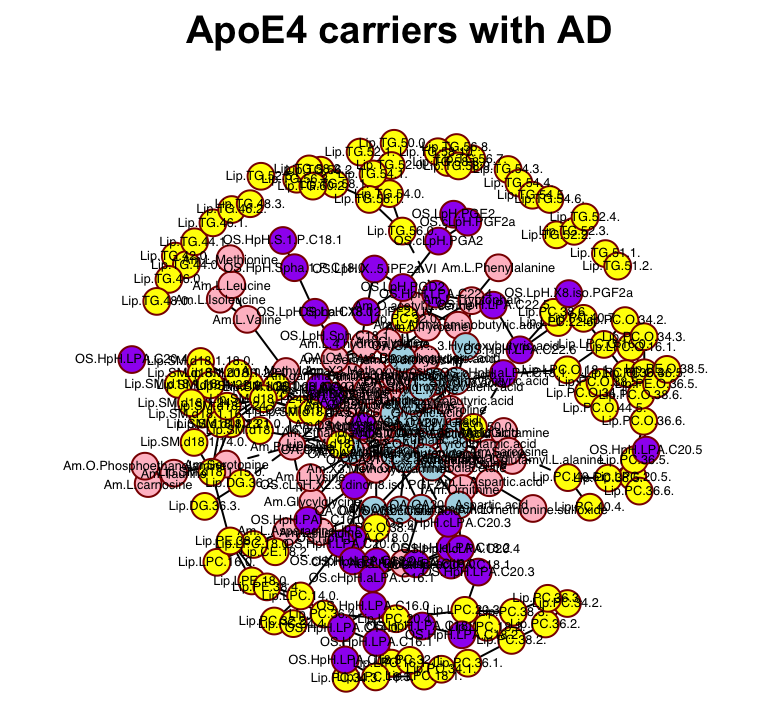
\includegraphics[width=\linewidth]{figures/netAD.png}
    a
  \endminipage\hfill
  \minipage{0.32\textwidth}
    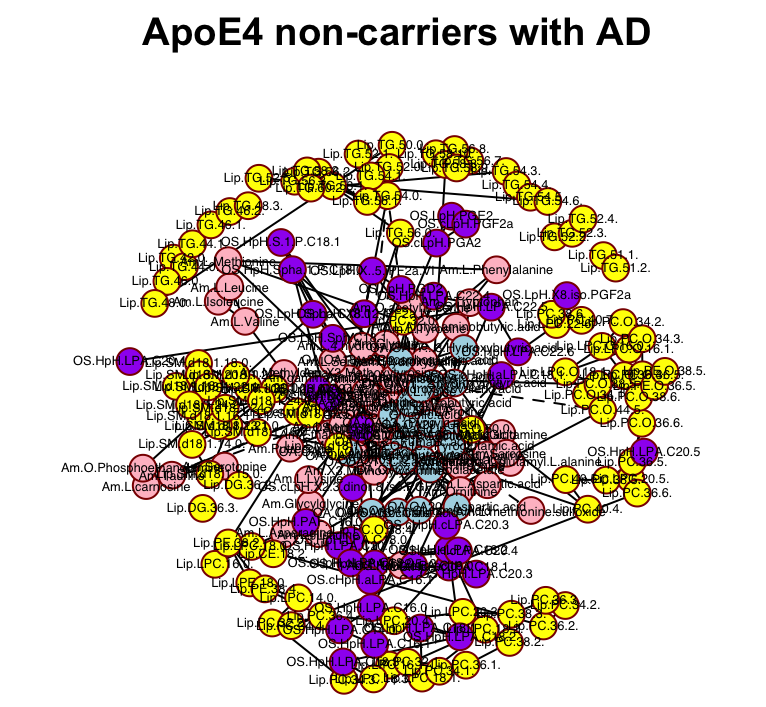
\includegraphics[width=\linewidth]{figures/netSCD.png}
    b
  \endminipage\hfill
  \minipage{0.32\textwidth}
  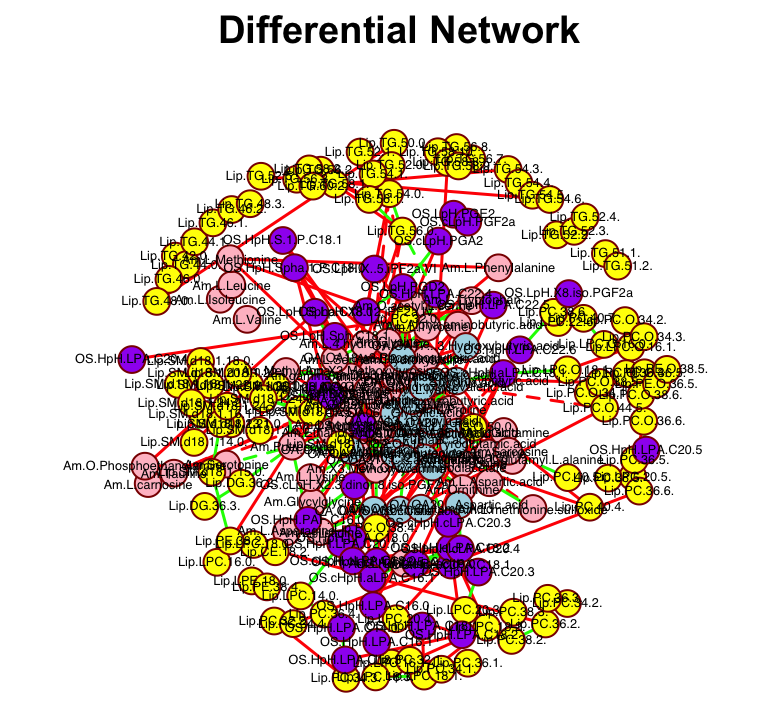
\includegraphics[width=\linewidth]{figures/netDiff.png}
  c
  \endminipage
\caption{Prunned metabolite covariance network topologies among ApoE4 carriers (a) and non-carriers in AD (b); differential edge network (c). The ApoE4-positive metabolite covariance network is more sparse compared to ApoE4-negative. Red edges represent links that are present exclusively in ApoE4 carriers. Green edges represent connections found in ApoE4 non-carriers.}  
  \end{figure}
\clearpage
\section{Discussion} \label{discuss}

\clearpage
\section{Conclusion} \label{concl}


%--------------- Main matter ----------------------------------------
%--------------------------------------------------------------------




%--------------------------------------------------------------------
%--------------- References -----------------------------------------
\newpage
\section*{References}
\printbibliography[heading=none]
\clearpage
%--------------- References -----------------------------------------
%--------------------------------------------------------------------
\appendix 
\clearpage
\section{Multiclass ROC curves}
\begin{figure}[htb]
  \includesvg[width=.75\textwidth]{figures/tree.svg}
  \caption{ROC curves of Decision Tree fitting the 6 ML-estimated latent factors on top of the clinical background variables, obtained from repeated (100 times) 10-fold CV}
  \label{roc:tree}
  \includesvg[width=.75\textwidth]{figures/xgb.svg}
  \caption{ROC curves of Xtreme Gradient Booster fitting the 6 ML-estimated latent factors on top of the clinical background variables, obtained from repeated (100 times) 10-fold CV}
  \label{roc:xgb}
  \end{figure}
\section{R Session Information} \label{appendixB}

\begin{verbatim}
R version 4.3.2 (2023-10-31)
Platform: aarch64-apple-darwin20 (64-bit)
Running under: macOS Sonoma 14.2.1

Matrix products: default
BLAS:   .../vecLib.framework/Versions/A/libBLAS.dylib 
LAPACK: LAPACK version 3.11.0

locale:
[1] en_US.UTF-8

time zone: Europe/Amsterdam
tzcode source: internal

attached base packages:
[1] stats     graphics  grDevices datasets  utils     methods   base     

other attached packages:
 [1] rags2ridges_2.2.7       nnet_7.3-19             DMwR2_0.0.2                       
 [4] dplyr_1.1.4             caret_6.0-94            lattice_0.21-9                    
 [7] globaltest_5.56.0       survival_3.5-7          heatmaply_1.5.0               
[10] xgboost_1.7.6.1         pROC_1.18.5             FMradio_1.1.1       
[13] future_1.33.0           ggthemes_5.0.0          corpcor_1.6.10
[16] viridisLite_0.4.2       plotly_4.10.3           ggplot2_3.4.4
[19] rpart_4.1.21            furrr_0.3.1             viridis_0.6.4 
[22] e1071_1.7-14            

loaded via a namespace (and not attached):
  [1] splines_4.3.2           bitops_1.0-7            tibble_3.2.1                              
  [4] XML_3.99-0.16           lifecycle_1.0.4         globals_0.16.2                            
  [7] magrittr_2.0.3          Hmisc_5.1-1             rmarkdown_2.25                        
 [10] lubridate_1.9.3         zlibbioc_1.48.0         sfsmisc_1.1-16                                 
 [13] RCurl_1.98-1.13         ipred_0.9-14            lava_1.7.3                               
 [16] S4Vectors_0.40.2        listenv_0.9.0           gRbase_2.0.1                                
 [19] codetools_0.2-19        tidyselect_1.2.0        TSP_1.2-4                                             
 [22] jsonlite_1.8.8          Formula_1.2-5           iterators_1.0.14                     
 [25] snowfall_1.84-6.3       Rcpp_1.0.11             glue_1.6.2                           
 [28] tufte_0.13              TTR_0.24.4              GenomeInfoDb_1.38.2         
 [31] fastmap_1.1.1           fansi_1.0.6             digest_0.6.33                  
 [34] RSQLite_2.3.4           utf8_1.2.4              tidyr_1.3.0                  
 [37] recipes_1.0.9           class_7.3-22            httr_1.4.7                      
 [40] gtable_0.3.4            timeDate_4032.109       blob_1.2.4                     
 [43] RBGL_1.78.0             GSEABase_1.64.0         scales_1.3.0                        
 [46] knitr_1.45              rstudioapi_0.15.0       tzdb_0.4.0                         
 [49] curl_5.2.0              proxy_0.4-27            cachem_1.0.8                     
 [52] foreign_0.8-85          AnnotationDbi_1.64.1    pillar_1.9.0                        
 [55] VGAM_1.1-9              xtable_1.8-4            cluster_2.1.4                       
 [58] cli_3.6.2               compiler_4.3.2          rlang_1.1.2                     
 [61] plyr_1.8.9              stringi_1.8.3           assertthat_0.2.1               
 [64] Matrix_1.6-1.1          hms_1.1.3               bit64_4.0.5                      
 [67] quantmod_0.4.25         bit_4.0.5               hardhat_1.3.0 
 [70] graph_1.80.0            xts_0.13.1              MASS_7.3-60 
 [73] dendextend_1.17.1       backports_1.4.1         yaml_2.3.8   
 [76] DBI_1.1.3               RColorBrewer_1.1-3      expm_0.999-8   
 [79] purrr_1.0.2             BiocGenerics_0.48.1     seriation_1.5.4 
 [82] IRanges_2.36.0          RSpectra_0.16-1         GenomeInfoDbData_1.2.11
 [85] annotate_1.80.0         parallelly_1.36.0       stats4_4.3.2 
 [88] foreach_1.5.2           tools_4.3.2             snow_0.4-4
 [91] prodlim_2023.08.28      gridExtra_2.3           xfun_0.41 
 [94] ca_0.71.1               withr_2.5.2             BiocManager_1.30.22
 [97] timechange_0.2.0        R6_2.5.1                colorspace_2.1-0
[100] generics_0.1.3          renv_1.0.3              data.table_1.14.10
[103] htmlwidgets_1.6.4       ModelMetrics_1.2.2.2    pkgconfig_2.0.3
[106] registry_0.5-1          XVector_0.42.0          htmltools_0.5.7
[109] Biobase_2.62.0          png_0.1-8               gower_1.0.1
[112] reshape2_1.4.4          checkmate_2.3.1         nlme_3.1-163
[115] zoo_1.8-12              stringr_1.5.1           parallel_4.3.2
[118] grid_4.3.2              reshape_0.8.9           vctrs_0.6.5
[121] htmlTable_2.4.2         evaluate_0.23           readr_2.1.4
[124] crayon_1.5.2            future.apply_1.11.0     fdrtool_1.2.17 
[127] munsell_0.5.0           Biostrings_2.70.1       lazyeval_0.2.2 
[130] KEGGREST_1.42.0         igraph_1.6.0            memoise_2.0.1 
[133] base64enc_0.1-3         webshot_0.5.5
\end{verbatim}



\end{document}



% This is a template for a thesis at Biometris created by C.F.W. Peeters in 2021 